\chapter{Scout: System Design and Implementation}
\label{chapter:scout}

To solve the CAT problem,
one-shot prediction (such as \paris~\cite{Yadwadkar2017}) suffers from
high variance of prediction error
while \bo (such as \cherrypick~\cite{Alipourfard2017} and \arrow~\cite{Hsu2018Arrow},
described in Chapter~\ref{chapter:arrow}) must
tolerate the \emph{cold-start} issue.
In this chapter, we design and implement an
effective, efficient and reliable system that recommends
the best architectural configurations 
that satisfies performance and cost objectives
to run a given workload.


\section{Introduction}
\label{ch4:sec:introduction}

Many storage systems are moving away from dedicated appliance-based storage model to software-defined 
storage (SDS), which separates software that provisions and manages storage from the hardware that provides raw physical storage~\cite{sds_att, Thereska2013, Jalaparti2012}.
This trend is partly driven by the tremendous growth of data and the emergence of cloud applications that operate in a multi-tenant environment with diverse workload characteristics.
As a result, the rigid appliance-based model, with tightly-coupled hardware and software features, is no longer cost-effective, lacks flexibility, and does not scale well.
SDS systems are increasingly abandoning centralized storage services in favor of distributed systems like Ceph~\cite{ceph}, HDFS~\cite{hadoop}, Swift~\cite{openstack}. 
Distributed storage systems are attractive because they scale well, allowing storage services to grow or shrink, based on storage demands. 
They are also better suited to handle diverse multi-tenant workloads. 

Providing reliable quality of service (QoS) to storage applications is critical in an SDS environment shared by multiple applications 
with diverse usage patterns. However, in a distributed storage environment, it is challenging to provide storage QoS in a consistent 
and reliable manner. Practical deployments of modern distributed storage systems like Ceph are composed of a large number of 
individual storage components that can interact in a complex manner. 
Diverse and time-varying storage workloads and performance interference in a multi-tenant environment further 
complicate the reliable assurance of storage QoS. Reliable and accurate monitoring of 
high-level storage performance metrics (e.g. throughput and IOPS) is critical 
for providing storage QoS guarantees.    
However, monitoring end-to-end storage performance is difficult in a distributed storage service. 
Instrumenting user applications to measure storage performance is not always practical. 
Performing benchmark tests in production systems also has practical limitations since they 
interfere with storage application workload.
Furthermore, running exhaustive benchmark experiments to cover diverse application workloads, 
deployment topologies, and large configuration parameter space is time-consuming and impractical in many cases. 
Building accurate analytical performance models, on the other hand, is also difficult for the reasons mentioned above.
 
This chapter proposes the idea of using low-level system metrics (e.g., CPU usage, RAM usage and network I/O)
as a proxy for measuring high-level performance (e.g., end-to-end IOPS and throughput) of 
distributed storage applications.
We design, implement and evaluate a practical tool, called \emph{Inside-Out}, that applies 
machine learning techniques to the low-level metrics collected from individual components 
of a distributed storage system to accurately estimate high-level storage performance metrics---like throughput and IOPS---of the entire 
distributed storage system.
We believe that a tool like Inside-Out can serve as an important component of the overall SDS architecture.

Inside-Out takes a black-box modeling approach, which does not require knowledge about distributed storage system protocol, workload characteristics, and deployment topology. 
Inside-Out relies upon machine learning techniques to automatically derive an accurate end-to-end performance model.
We explore several well-known machine learning algorithms including linear regression, 
decision tree learning, and ensemble methods \cite{Wang2004, Noorshams2013}, and conclude that  
there does not exist an one-size-fits-all algorithm that can work in all prediction cases.
Hyperparameter tuning \cite{Chapelle2002, Noorshams2013}, model selection \cite{Kohavi1995} and 
feature selection \cite{guyon2003introduction, Saeys12007} all turn out to be too complicated for optimizing prediction accuracy.
In contrast, Inside-Out uses a two-level learning method that automatically selects important features, boosts prediction accuracy, and achieves consistent prediction. 
This two-level learning method pipelines two supervised learning algorithms to eliminate irrelevant features while avoiding overfitting problems.\footnote{\label{ft:overfitting}
Overfitting describes the situation when a model captures the relationship of noisy data but not the underlying relationship \cite{domingos2012few}.
Overfitting becomes more prominent in the presence of high dimensional data}

Inside-Out offers several key benefits. 
%[MRA] Unlike traditional analytic performance modeling approach, Inside-Out is generic in nature, and therefore, it can be applied to different storage services.  
Unlike traditional analytic performance modeling approach, Inside-Out is more generic, 
and therefore can be more easily applied to different storage services.  
Different from previous work, Inside-Out 
does not require information about system configuration and application workload~\cite{Ruemmler1994, Shriver1998, Wang2004, Kelly2004, Yin2006, Noorshams2013, Ardagna2014}. 
Due to the self-learning property, \emph{Inside-Out} improves performance prediction accuracy with more data.
It can also adapt to changes in the system
by continuously learning the system behavior. 

We evaluate Inside-Out using Ceph~\cite{ceph} %as an example distributed storage system 
running on an OpenStack-based SDS platform.
The low-level performance metrics are collected from participant virtual machines 
running various components of a Ceph storage service.\footnote{\label{ft:vm}
Our approach is not limited to VM-based environments.
It can be applied to container-based and bare-metal storage servers as well.
}
Our in-depth evaluation shows that Inside-Out generates end-to-end performance models with 91.1\% prediction accuracy on average.
More importantly, as discussed above, Inside-Out is generic in nature as it captures the behavior of the storage system 
by analyzing low-level system metrics (that are protocol and application agnostic). Furthermore, we demonstrate that Inside-Out 
%[MRA] can provide reliable performance monitoring even in the presence of evolving workload characteristics, changing storage 
can provide reliable hints for performance monitoring tasks even in the presence of evolving workload characteristics, changing storage 
configuration and interfering tenants. We also show that Inside-Out is reliable in estimating end-to-end performance 
even when the storage system expands or shrinks.
We show that Inside-Out provides reliable performance 
prediction when the storage system is up to four times larger than the one used for building machine learning models during 
the training phase. 
Lastly, Inside-Out is able to learn new storage behavior over time.
%\section{Why Collective Optimization}
\label{sec:motivation}

A cloud optimizer is often evaluated with search performance and measurement cost.

\begin{itemize}
\item \textbf{Search performance} is the measure of the quality of the found solutions by an optimizer.
For example, in searching for the most cost-effective configuration, an optimizer that finds a configuration that is only 10\% more expensive than the optimal is considered better than another optimizer
that can only find a configuration that yields 30\% more cost.
Therefore, we use normalized performance (to the optimal) for evaluation.

\item \textbf{Search cost}
is the total cost of running an optimizer.
An optimization process is expensive because it requires
to test a workload on some cloud configurations for deriving
the best choice.
We use the number of tests as the search cost (or measurement cost)
because it is an intuitive measure.
The amount of charge is another measure~\cite{Alipourfard2017}. 

\end{itemize}


There is always a trade-off between measurement cost and search performance.
The primary motivation for collective optimization is to reduce high measurement cost of optimizing multiple workloads.
If users demand strict search performance, they better turn to single-optimizers.
However, we argue that collective optimization is promising
because it achieves comparable or slightly worse search performance
while reducing measurement cost significantly.
In the following,
we discuss the benefits of having a collective optimizer.


\begin{itemize}
\item \textbf{Large scale cloud migration.}
Cloud computing is a cost-effective solution.
Enterprises are moving in-house applications to the cloud,
and need a quick way for large migration~\cite{khajeh2010cloud,sripanidkulchai2010clouds}.
Elaborate optimizers are expensive (in measurement cost) and time-consuming (in optimization process).

\item \textbf{Limited budgets.}
The single-optimizer such as \emph{CherryPick} and \emph{Scout} are effective and desirable for highly recurring workloads because the measurement cost can be amortized.
However, the number of budgets to run optimizers
does not increase linearly with the number of workloads.
To better support multiple workloads,
we need to reduce measurement cost while delivering comparable search performance.

\item \textbf{Expanding cloud portfolio.}
Cloud providers expand their cloud portfolio more than 20 times in a year~\cite{ec2history}.
Therefore, users have to rerun optimizers to update their configurations for all workloads.
Again, this is an expensive and time-consuming process.

\item \textbf{Seed cloud optimizers.}
All the cloud optimizers require initial measurements.
It is unclear how to determine the best starting points.
We aim to find the exemplar configurations,
which can be used as the starting points, thereby
reducing measurement cost.
The exemplar configuration can be used to seed singe-optimizers such as CherryPick and \scout, which will be discussed more in Section~\ref{sec:system}.

\end{itemize}

In summary, users would prefer collective optimization if search performance is comparable to single-optimizers while measurement cost can be reduced greatly.

\section{Design Choices}
\label{sec:design}

\begin{figure}
\resizebox{.8\linewidth}{!}{%
    \small{
        \begin{tabular}{@{}lccccc@{}}
        \toprule
        \textbf{Methods} & \textbf{\begin{tabular}[c]{@{}c@{}}Search-\\ based\end{tabular}} & \textbf{\begin{tabular}[c]{@{}c@{}}Relative\\ Ordering\end{tabular}}  & \textbf{\begin{tabular}[c]{@{}c@{}}Low-level\\ Metrics\end{tabular}} & \textbf{\begin{tabular}[c]{@{}c@{}}Historical\\ Data\end{tabular}} & \textbf{\begin{tabular}[c]{@{}c@{}}Transfer\\ Learning\end{tabular}} \\ \midrule
        CherryPick~\cite{Alipourfard2017} & \cmark & \xmark & \xmark & \xmark & \xmark \\
        PARIS~\cite{Yadwadkar2017} & \xmark & \xmark & \cmark & \cmark & \xmark \\
        Arrow~\cite{Hsu2018Arrow} & \cmark & \xmark & \cmark & \xmark & \xmark \\
        \cellcolor[HTML]{9B9B9B}\textcolor{white}{\textbf{Scout}} & \cellcolor[HTML]{9B9B9B}\color{white}\cmark & \cellcolor[HTML]{9B9B9B}\color{white}\cmark & \cellcolor[HTML]{9B9B9B}\color{white}\cmark & \cellcolor[HTML]{9B9B9B}\color{white}\cmark & \cellcolor[HTML]{9B9B9B}\color{white}\cmark \\ %\bottomrule
        \end{tabular}
    }
    }
    \centering
    \caption{
    \small{
    \textbf{An overall comparison with other CAT methods.}
    A search-based method better tolerates prediction bias.
    Relative ordering better captures the workload-architecture-performance relationship.
    Leveraging low-level metrics improves search performance.
    Historical data helps eliminate unnecessary exploration overhead in a search.
    Transfer learning greatly reduces search cost.}
    }
    \label{fig:model_classification}
\end{figure}


By analyzing the differences between the state of the art methods,
we identified the following key components in solving the CAT problem:
(1) a search-based method (similar to \emph{Cherrypick}~\cite{Alipourfard2017})
is essential since it accommodates mispredictions and performance variances
in the cloud,
(2) relative ordering better captures
the workload-architecture-performance relationship,
which creates fewer mispredictions,
(3) low-level performance metrics are a good proxy of
predicting system performance~\cite{Novakovic2013,Hsu2016,Yadwadkar2017},
(4) historical data (as used in PARIS~\cite{Yadwadkar2017}) is useful
to understand the inherent preferences of a workload, and
(5) transfer learning boosts search performance and improves convergence speed
by minimizing exploration phase.
These components together solve the CAT problem more effectively
and overcome the shortcomings of the current state of the art approaches.
\myfigure{\ref{fig:model_classification}} compares and contrasts the
design choices of \scout against prior work.

Because it is a daunting task to build an accurate model that
predicts performance and cost of workloads on
distinct cloud architectural configurations,
we can instead build an indirect model (for improving prediction accuracy).
A search-based method does not require a direct answer
(which choice is the best),
but an answer to ``are there better choices?''
We do not predict the absolute performance of a configuration but rather
predict the relative performance of two configurations.
That is, we can simplify the prediction model that will assist
a search-based method in finding the solutions more efficiently~\cite{nair2017}.
\emph{Learning to rank} is an important machine learning task
~\cite{harrell2001ordinal,li2008mcrank,cao2007learning}.
We prefer relative ordering instead of total ordering for
ranking architectural configurations because
there does not exist a one-size-fits-all architecture
for any workloads and for any objectives.

SMBO requires exploration efforts
(increases search cost)
to update its belief (prediction) on the search space.
However, the data for the initial model need not come from
the workload being evaluated.
Rather, data from any workload can be used to build a useful model describing
the search space.
For this model to be most useful, the information must be generic---independent
of workloads.
This technique is inspired by \cite{Hsu2016,Yadwadkar2017}.
There are too few features (dimensions and options) in the configuration space
to build a robust model that works across many workloads.
Consequently, a model based only on architectural features
(\eg{cluster sizes and memory per core}) is fragile.

To summarize, the following elements are necessary
to create an effective approach.
\begin{enumerate}[leftmargin=*]
    \setlength\itemsep{-0.4em}
    \item Prefer the \textbf{\textit{search-based technique}}, which converges to the best solution iteratively and avoids the large penalty caused by dramatic prediction error.
    \item Use a \textbf{\textit{relaxed}} model that boosts prediction accuracy, thereby better guides a search process to find the near-optimal configurations more quickly,
    \item Use \textbf{\textit{low-level metrics}} to generate a generic representation of the search space such that it can be used by other combinations of workload and application.
    \item Create a \textbf{\textit{performance database}} so that the knowledge of optimization can be used by other optimizers to find the right cloud configuration and hence reduce the search cost. 
\end{enumerate}
\section{From Observation to Action}
\label{sec:approach}
In this section, we describe how to derive search hints from performance data
to guide a search process.

\subsection{Exploration vs. Exploitation}

A search-based method navigates in the search space
to find the best cloud architectural configuration.
It is mostly concerned with
two questions:
``what are better choices?'' and
``what are more promising regions?''
The former ensures that a search will
eventually, find a near-optimal configuration
while
the latter determines how quickly it finds the solution
(also known as convergence speed).
An effective and efficient search method must answer
these two questions.

To this end, we actually need only to know ``what are better choices?''
At each step, a search-based method aims to find a cloud configuration
that is better than the current best.
A higher probability of \emph{guessing} the next step right
ensures that a search process sequentially finds a better choice.
A right next step also guides a search process
to move towards the right direction.
As long as the optimizer can move closer to the desired solution at each step,
it is more likely to guarantee it will find
near-optimal solutions.

To better determine the next step, a search process can learn
from the observations along the search path.
However, this method faces two challenges.
First, it requires collecting sufficient data to build strong belief.
\emph{CherryPick} is confronted by the cold-start issue
since it must first explore the search space---to identify the promising regions.
Second, an insufficient number of observations leads to
high bias in prediction---the method can wrongly believe that
a particular region (such as VM types or cluster sizes) is more promising
than the other, leading to a sub-optimal solution.

Instead of learning only from observations collected
while executing the target workload, a search process also can learn from
performance data of other workloads---which have been optimized in the past.
This addresses the issue of high bias because a larger number of
measurements (performance data) is available to create a prediction model that
generalizes a performance model better.
This also sidesteps the exploration problem because the search process
does not need to collect observations by running workloads
of the current search task.
The idea of reusing the data is often tricky
since the different combination of application and workload exhibit
very different behavior.
For example, the same application with different inputs can create
very different workload behavior
(such as the execution time and running cost)~\cite{Hsu2018Arrow}.
A performance model, which captures this complex behavior requires
more information about the search space than just
the architecture level information such as VM types and cluster sizes.


\subsection{Core Techniques}
To navigate the search space efficiently, \scout is built on
the following four ideas.


\subsubsection*{Pairwise comparison}
A search-based method determines the next configuration to evaluate.
That is, the method only needs to rank
the set of unevaluated cloud configurations.
Therefore, we can use \textit{Pairwise Comparison} modeling scheme~\cite{wauthier2013efficient}.
\emph{CherryPick} uses Gaussian process to build prediction model,
$f(x_i, K) = y_i$, where $x_i$ is the feature vector to represent
an architecture configuration and $K$ is the covariance kernel function.
With pairwise comparison, the learning task is
\begin{equation} \label{eq:1}
f(x_i, y_i, x_j) = y_j,
\end{equation}
where $x_i \in E$ and $x_j \in S-E$.
In words, it predicts the cost ($y_j$) of a configuration not yet
evaluated ($x_j$) given the cost ($y_i$) from the best configuration
yet found ($x_i$).
This modeling technique does not require to make an assumption ($K$) about
the search space (which is another hyper-parameter to tune),
and
naturally fits into SMBO in updating belief upon new observations.
For the same workload, switching
from a smaller VM type (\eg{\emph{large}}) to a larger one (\eg{\emph{2xlarge}})
may result in different performance on different VM families
(\eg{\emph{c4} and \emph{r4}}).
This performance relationship may change dramatically due to workload changes.
Regression-based modeling needs to fit the corresponding features accurately
for predicting performance~\cite{rasmussen2004gaussian,wettschereck1997review}.
Pairwise comparison helps capture performance transition
between architectural configurations.
Although there are $P(n,2)$ pairs (permutation),
where $n$ is the number of configurations,
in practice, we do not have to obtain full pairs for training this model.
This is because some pairs, \eg{(\emph{c4.large}, \emph{r4.large})}, show
significant performance differences in comparison with other pairs,
\eg{(\emph{m4.large}, \emph{r4.large})}.

\subsubsection*{Relative ordering}
Ranking architectural configurations does not need to predict
absolute performance (a harder problem).
Besides, ``a bad learner'' sometimes can still find a good solution~\cite{nair2017}. 
The idea of using an inaccurate model is useful
because the effort required to build an accurate model is much higher than
an inaccurate model.
%Hence, we do not need to predict performance directly rather
%the relative ordering or ranks.
%\ick[redundant with above?]
Based on this insight, we choose not to infer (inaccurate) performance measure
but rather to infer (accurate) relative ordering---
one configuration is better than another.
To support relative ordering, we modify the learning task from
\myequation{\ref{eq:1}} to
\begin{equation} \label{eq:2}
f(x_i, x_j) = \sigma({\frac{y_j}{y_i}})
\end{equation}
where $\sigma$ is a ranking function.
Binary ranking (\ie{better or worse}), for example, is the simplest form.
This transformation simplifies the learning task because
it does not predict absolute performance.
Furthermore, a coarse-grain ranking function better tolerates
performance variance in the cloud because
a small variance may still result in the same ranks.
%This technique trades search cost for search performance.
\myfigure{\ref{fig:reg_clas}} shows that the prediction accuracy of
relative ordering (using classification) is higher than
total ordering (using regression).
This experiment uses \emph{ExtraTrees}~\cite{geurts2006extremely} in
both the regression and classification task for fair comparison.
The increase in prediction accuracy greatly reduces search cost because
it is more likely to avoid wrong predictions (see Section~\ref{sec:why_better}).


\subsubsection*{Low-Level Insight}
Low-level performance metrics help identify
performance problems~\cite{Bodik2010, Novakovic2013} and
predict application and system performance~\cite{Hsu2016,Yadwadkar2017}.
Understanding resource bottlenecks helps choose the right cloud configuration and helps \scout ignore not so promising cloud configurations.
For example, in optimizing execution time, a memory bottleneck indicates
an instance with larger memory may improve resource efficiency,
thereby reducing execution time.
With low-level performance information, our learning task becomes
\begin{equation} \label{eq:3}
f(x_i, m_i, x_j) = \sigma({\frac{y_j}{y_i}})
\end{equation}
where $m_i$ represents the low-level performance vector.
This is similar to the process of
troubleshooting performance problems and
identifying resource bottleneck.
Instead of constructing rules manually,
this learning task can extract those rules implicitly.
When a workload runs inefficiently on one architectural configuration,
\scout observes abnormal or insufficient resource usage.
This observation is translated to prediction probability implicitly.
\scout ignores those configurations with low prediction probability.


\subsubsection*{Transfer learning}
The accuracy of a performance model depends on the number of data points
used to train the model.
In CAT, the data points are expensive to compute.
When building the performance models, it might be best to reference observations
from other optimization processes.
Researchers in transfer learning report that data
from other optimization processes can yield better models
than just using current data~\cite{pan2010survey,peters2015lace2}.
In this work, workloads share the same search space $S$ and therefore,
architectural features are the same.
Besides, \scout uses generic low-level metrics.
These enable transfer learning possible in \scout.
Although including workload information might improve search performance,
it prevents \scout from transferring knowledge
from historical optimization data.

\begin{figure}[t]
 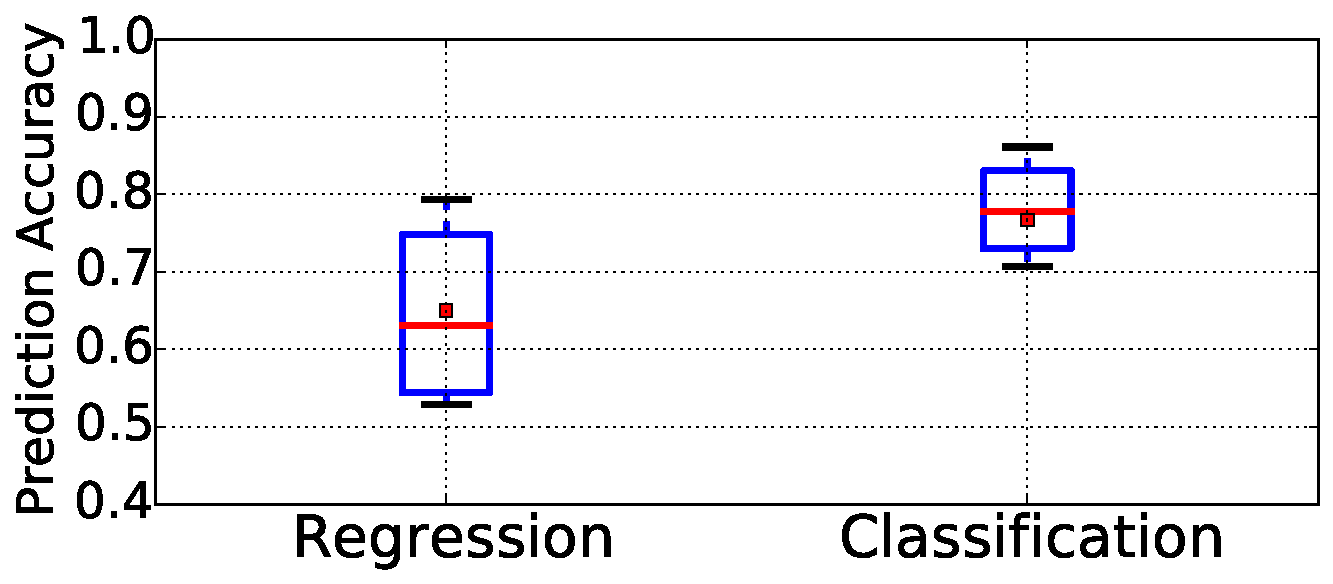
\includegraphics[width=.8\textwidth]{figures/multiple_prediction_accuracy.pdf}
 \centering
 \caption{\textbf{On the model selection of predicting the next step.}
 We evaluate the ability to distinguish a good and a bad configuration.
 In regression, we test rank preserving as prediction accuracy~\cite{nair2017}.}
 \label{fig:reg_clas}
\end{figure}


\subsection{Search Hints}
This section explains how to extract search hints using
probabilistic classification methods
~\cite{friedman2001elements,zadrozny2001obtaining,zadrozny2002transforming}.
A probabilistic classifier predicts probability distribution over
predicted classes.
In \myequation{\ref{eq:3}}, the learning task ranks the relative
performance measure of two architectural configurations.
We can map ranks to classes.
For example, the rank function $\sigma$ outputs \emph{class 1} if
$\frac{y_j}{y_i} < 1.1$. Otherwise, the output is \emph{class 0}.
A binary classifier is able to answer ``is $x_j$ better than $x_i$?''
A probabilistic classifier outputs higher probability for \emph{class 1} if
a specific workload performs better on $x_j$ than $x_i$.

We use an example to illustrate this process.
Consider a configuration space ($S=\{S_1, S_2, S_3, S_4\}$).
An CAT optimizer starts with $S_1$ and $y_1 = \phi(S_1) = 10$ (the current best).
Let us assume we have collected historical data for
training the probabilistic classifier.
The predicted probability distribution over ${S_1, S_2, S_3, S_4}$ 
is $[-, 0.8, 0.2, 0.2]$.
The probability vector $P_{i}$ represents
``how likely $S_j$ is a better choice than $S_i$.''
A higher value indicates $S_j$ is more likely
to perform better than $S_i$. 
In this example, $S_2$ is a better choice than the others.
When the actual performance measure is better $\phi(S_2) \leq \phi(S_1)$,
then CAT optimizer found a better solution than the current best.

The above example uses a binary classifier, and
\scout uses multiclass classification.
The intuition for using multiple classes is that some configurations
yield similar performance, and \scout should not consider little improvement.
For example, we can define the classes to be ``better,'' ``fair,'' and ``worse.''
\scout favors the configurations in the ``better'' class.
\scout uses a predefined discretization policy
(based on user-defined thresholds)  to convert probability to discrete classes.
%For example, $\frac{\phi(S_j)}{\phi(S_i)} \leq 0.8$ is considered as ``better.''
%\ick[do you mean i is better?]


\subsection{Search Strategy}

During the search process, a new observation
(running a workload on a selected cloud configuration)
provides the necessary information to determine
whether there exist better choices (see \myequation{\ref{eq:3}}).
The probability vector $P_{i}$ is derived
for each new observation $\phi(S_{i})$.
A search strategy determines the choice based on the probability predictions.
At each step, the search process selects the configuration $S_j$ with
the maximum probability in $P_{i}$.

This search strategy is similar to depth-first search.
While \emph{CherryPick} requires balancing exploration and exploitation,
\scout tends to exploit---because it uses historical data.
When the prediction model can generate quality predictions,
this search strategy leads to quick convergence speed
(the selected configuration improves over the current best).
Therefore, the search process has low search cost to find near-optimal
configurations. 

A search process should stop when it no longer can find a better configuration. This is controlled by a predefined parameter called  \textit{probability threshold} ($\alpha$) and acts as a stopping criterion.
When the predicted probability $P_{ij}$ is lower than $\alpha$ for all $S_j$,
the search process is not confident that it would find better configurations in the next step.
A search should also stop if it fails to find better solutions due to an inaccurate performance model. This is controlled by another parameter called \textit{ misprediction tolerance} ($\beta$) to avoid excessive search cost.

\subsection{Putting It All Together}
We have shown that the core element of a search based method is to determine
the next best step.
For obtaining hints to guide a search process,
we propose using the probabilistic classification technique
to predict improvement probability.
That is similar to Expected Improvement (EI) in \emph{CherryPick}.
We choose pairwise comparison and relative ordering
to deliver high prediction accuracy and to naturally into the search process.
\scout leverages low-level performance information and
extracts rules (based on resource utilization) implicitly.
This improves a search process because certain types of cloud configurations
can be avoided (as we will show in Section~\ref{sec:evaluation}).
Last, we choose a search strategy that merely picks the configuration
that is most likely to be better than the current best.
This strategy increases convergence speed---has low search cost.

\section{To Eliminate Sub-Optimal Choices}
\label{sec:system}

While the exemplar configuration is adequate for most workloads and reduces measurement cost significantly, it is almost inevitably that fewer workloads may suffer from sub-optimal performance (since we trade-off near-optimal performance for a large reduction in measurement cost).
For instance, 30\% workloads (\textit{c4.large}) underperform ($> 1.4$) as shown in \mytable{\ref{table:top3}}.
Similarly, the 90 percentile in \myfigure{\ref{fig:s2_cost_performance}}.
Although we have shown \micky is much more practical in the knee point analysis (Section~\ref{sec:kneepoint}),
it would be great if we can inform users of those sub-optimal choices.


We propose a two-level approach that integrates our previously built system, \scout, to detect this problem for further optimization~\cite{Hsu2018Scout}.
\scout is able to answer ``is there a better configuration than the current choice?''.
\myfigure{\ref{fig:system_design}} illustrates the proposed system integration.
Users get choices of optimizing those under-performed workloads.
\myfigure{\ref{fig:detection_misprediction}} indicates that those sub-optimal choices are very likely to be identified.
The detection module can detect bad performance with a median accuracy of 98\%.
This is promising because users benefit from
low measurement cost (by \micky) and
performance guarantee (by \scout).
This ability enables users to further optimize for those sub-optimal workloads, which is particularly beneficial to highly recurring workloads.

\section{Evaluation}
\label{sec:evaluation}

%In this section, we present a comprehensive evaluation of how well Inside-Out can predict end-to-end storage performance (latency, throughput and IOPS) 
%using low-level system metrics for a wide range of SDS environment.
In this section, we present a comprehensive evaluation of Inside-Out.
We demonstrate that Inside-Out can accurately predict end-to-end performance, 
i.e., throughput and IOPS, using low-level system metrics and
is applicable to a wide range of realistic scenarios.

%SDS offers wide flexibility for hosting storage services and in this section, we present comprehensive evalution to study whether low-level performance metrics can accurate end-to-end performance and Inside-Out can be applied for practical use in many SDS senarios.
%All SDS scenarios are listed in Table~\ref{tab:prediction_scenario}.


\subsection{Setup}
\label{sec:dataset}

%We choose Ceph as the storage service running on our SDS platform \cite{ceph}. 
%We use COSBench for measuring the storage performance \cite{cosbench}.
%COSBench supports several object storage protocols, including \textit{librados} used by Ceph. 
We choose Ceph~\cite{ceph} as a target distributed storage service for our evaluation and             
use COSBench~\cite{cosbench} to generate various types of storage workloads.
COSBench supports several object storage protocols, including \textit{librados} for Ceph, and
provides a set of knobs to change storage traffic pattern. 
Table~\ref{tab:cosbench_configurations} lists Ceph and COSBench configurations used in our experiments.
%We collected benchmarking data from three SDS clusters 
%located in a research lab of a major telecommunication company. 

\newcommand{\scenarioMU}{Increasing users}
\newcommand{\scenarioCUB}{Complex usage}
\newcommand{\scenarioCRB}{Complex request}
\newcommand{\scenarioWIB}{Write intensive}
\newcommand{\scenarioRIB}{Read intensive}
\newcommand{\scenarioMWIB}{Medium write intensive}
\newcommand{\scenarioMRIB}{Medium read intensive}
\newcommand{\scenarioMM}{Reconfigure Ceph}
\newcommand{\scenarioSUI}{Scale-up instances}
\newcommand{\scenarioMBS}{Medium network SLO}
\newcommand{\scenarioLBS}{Low network SLO}
\newcommand{\scenarioSON}{Scale out to}
\newcommand{\scenarioSIN}{Shrink in to}
\newcommand{\scenarioMTA}{Case 1 - tenant 1 (250 Mbit)}
\newcommand{\scenarioMTB}{Case 1 - tenant 2}
\newcommand{\scenarioMTAA}{Case 2 - tenant 1}
\newcommand{\scenarioMTBB}{Case 2 - tenant 2}


\newcommand{\spheading}[2][10em]{% \spheading[<width>]{<stuff>}
  \rotatebox{90}{\parbox{#1}{\raggedright #2}}}

\begin{table*}[t!]
  \fontsize{8}{8}\selectfont
  \centering
  \caption{Common scenarios that storage behavior can change in a software-define storage environment}
  \begin{tabularx}{.95\linewidth}{|l|c|c|c|X|}
  \hline
  & \textbf{Scenario} & \textbf{Training Dataset} &  \textbf{Prediction Dataset} & \textbf{Explanation} \\
  \hline
  \multirow{7}{*}[-0.3ex]{\rotatebox[origin=c]{90}{\textbf{Changing Workload}}} & \scenarioMU & \{1, 2\} & \{4\} & The number of client virtual machines running COSBench. \\
  \cline{2-5}
  & \scenarioCUB & \{1, 2, 4, 8\} & \{16, 32\} & The number of threads for all benchmark clients. \\
  \cline{2-5}
  & \scenarioCRB & 512KB & 1-1024KB & The request size (either static or variable) of the workload, configured in COSBench. \\
  \cline{2-5}
  & \scenarioWIB & \{50, 75, 100\} & \{25, 0\} & \multirow{4}{1\linewidth}{The percentage of read operations the workload. The read and write percentages are 100 in total.}\\
  \cline{2-4}
  & \scenarioRIB & \{0, 25, 50\} & \{75, 100\} & \\
  \cline{2-4}
  & \scenarioMWIB & \{0, 50, 100\} & \{25\} & \\
  \cline{2-4}
  & \scenarioMRIB & \{0, 50, 100\} & \{75\} & \\
  \hline
  \hline
  \multirow{4}{*}[-1.7ex]{\rotatebox[origin=c]{90}{{\textbf{Reconfiguration}}}} & \scenarioMM & \{1\} & \{2\} & The number of Ceph monitor daemons.\\
  \cline{2-5}
  & \scenarioSUI & m1.small & m1.medium & The instance type of the virtual machines running Ceph is upgraded to a powerful one.  A m1.small instance has one core and 2GB memory and m1.medium has two cores and 4GB memory.  Note that in this setting, the configuration of disk I/O remains the same.\\
  \cline{2-5}
  & \scenarioMBS & unrestricted & 500 Mbps & The network bandwidth of virtual machines is limited at 500 Mbps.  We use the Linux tool \textit{tc} for network throttling\\
  \cline{2-5}
  & \scenarioLBS & unrestricted & 250 Mbps & Network bandwidth is limited at 250 Mbps.\\
  \hline
  \hline
  \multirow{2}{*}[-0.5ex]{\rotatebox[origin=c]{90}{\textbf{Elasticity}}} & \scenarioSON { \textit{n}} & \{4, 6, 8, 10\} & \{20, 30, 40\} & The total number of Ceph OSDs.  Note that each OSD is running in a virtual machine and different OSDs can run on the same physical servers (10 servers in total). \\
  \cline{2-5}
  & \scenarioSIN { \textit{n}} & \{20, 30, 40\} & \{4, 6, 8, 10\} & Similar to the above, but the cluster size is decreased. \\
  \hline
  \end{tabularx}
  \label{tab:prediction_scenario}
\end{table*}

\begin{table}[htp]
 \centering
 \caption{Ceph and COSBench settings for data collection.}
 \begin{tabular}{ ll  }
  \hline
  \textbf{\normalsize{Parameters}} & \textbf{\normalsize{Values}} \\
  \hline
  \textbf{Ceph version} & 9.2 (Infernalis) \\
  \textbf{\# of physical nodes} & 16 \\
  \textbf{Storage back end} & Logic Volume (iSCSI) \\
  \textbf{\# of storage nodes} & \{4, 6, 8, 10, 20, 30, 40\}\\
  \textbf{\# of drivers} & \{1, 2, 4\} \\
  \textbf{\# of workers} & \{1, 2, 4, 8\} \\
  \textbf{Request size} & \{512KB, 1-1024KB\} \\
  \textbf{Duration} & 180 sec \\
  \textbf{\# of containers} & \{64\} \\
  \textbf{\# of objects} & \{1024\} \\
  \textbf{read/write ratio} & \{100/0, 75/25, 50/50, 25/75, 0/100\} \\
  \hline
 \end{tabular}
 \label{tab:cosbench_configurations}
\end{table}



We collected benchmarking data from an OpenStack-based SDS platform.
The cluster has 16 machines, and
each machine has 16 cores, 24GB memory and 250GB disk space.
Each machine has 1Gbps network interface connected to a 10Gbps switch.
The dataset is collected from about 5300 benchmark runs. The total dataset is composed of about 15.2 million records, each of which is 
a vector of 32 low-level performance data.
The end-to-end performance data collected from COSBench contains 
3 million records. 
The combined dataset is about 24GB, collected over two weeks. 

%[comment: please briefly describe cluster A/B/C in text as well (using the table II's content). we need to be kind.]
%The dataset is collected from 8300 benchmark runs in total; 5300 runs on \textit{Cluster A}, 
%1500 runs on \textit{Cluster B}, and 1500 runs on \textit{Cluster C}.
%The total number of records of low-level performance data is more than 18 million 
%and each record is a vector with 32 metrics.
%Our resulting dataset is made up of 18 million records, each of which is 
%a vector of 32 low-level performance data.}
%The number of records for \chin{end-to-end} performance data collected from COSBench contains 
%\chin{3.6 million} records, which is one-fifth of the low-level records.
%The combined dataset is about 34GB, and is worth about two-week measurements in total.
%All raw performance data can be found at \chin{http://xxx.xxx}.
%RP: We cannot publish any data without approval from AT&T.


\subsection{The Comparison Method}
Our goal is to find a function $f(X_t)$ that predicts the end-to-end performance, where $X_t$ is a vector that describes the internal status at time $t$ of a distributed storage service.
We say a model is accurate if $f(X_t)=\hat{y_t} \simeq y_t$, where $y_t$ is the ground truth (measured at the client side) and $\hat{y_t}$ is the predicted values.
To interpret performance models, we are interested in four indicators:
1) the overall prediction accuracy,
2) the goodness-of-fit,
3) the consistency across diverse scenarios and
4) the consistency across prediction instances.

First, we use mean absolute percentage error (MAPE) to compute prediction accuracy as 
\setlength{\abovedisplayskip}{0pt} \setlength{\abovedisplayshortskip}{0pt}
%\begin{center}
\begin{equation} \label{eq:prediction_accuracy}
max(1 - \frac{\sum_{t=1}^{n} {|\frac{y_t - \hat{y_t}}{y_t}|}}{n}, 0)
\end{equation}
%\end{center}
where $n$ is the length of the observation period.
%For example, for a three-minute measurement period with one-minute sampling window, 
%if the measured performance values are $[10, 20, 30]$ and the predicted values are $[9, 18, 33]$, the average prediction accuracy is $90\%$.
We restrict the scope of prediction accuracy between $0$ to $1$ because the prediction accuracy can be negative (e.g. when $y_t$ is small).

Second, we use the coefficient of determination $R^2$ to interpret \emph{Goodness-of-Fit}, which is less than or equal to one \cite{Noorshams2013}.
Third, we examine whether a performance model can present consistent prediction in various SDS scenarios.
Last, we further analyze the probability density function of prediction decisions for different categories of prediction scenarios.

We consider prediction of throughput and IOPS for both read and write operations, and use the following terms $TP_r$, $TP_w$, $OP_r$ and $OP_w$ for read 
throughput, write throughput, read IOPS and write IOPS, respectively.



\subsection{Baseline: Prediction Performance on Static Deployment}
%

We evaluate prediction accuracy of Inside-Out under a variety of scenarios 
with different storage workloads and configurations
listed in Table~\ref{tab:prediction_scenario}.
In this subsection, we focus on a static deployment scenario with one storage tenant 
running on a distributed Ceph storage service that does not expand or shrink in terms 
of number of VMs used for running Ceph.
Later, we evaluate more challenging scenarios 
in which the Ceph cluster expands or shrinks based on user demand,
and storage traffic of multiple tenants interfere with each other.

%with the Ceph cluster expanding or shrinking based on user demand, 
%and multiple tenants interfering with each others storage traffic. 
%shows various scenarios where the prediction dataset differs from the training dataset.



\vspace{1ex}
%\subsection{Changing Workload}
\subsubsection{Can Inside-Out handle diverse workloads?}
\label{sec:changing_workload}

\begin{figure}
    \centering
    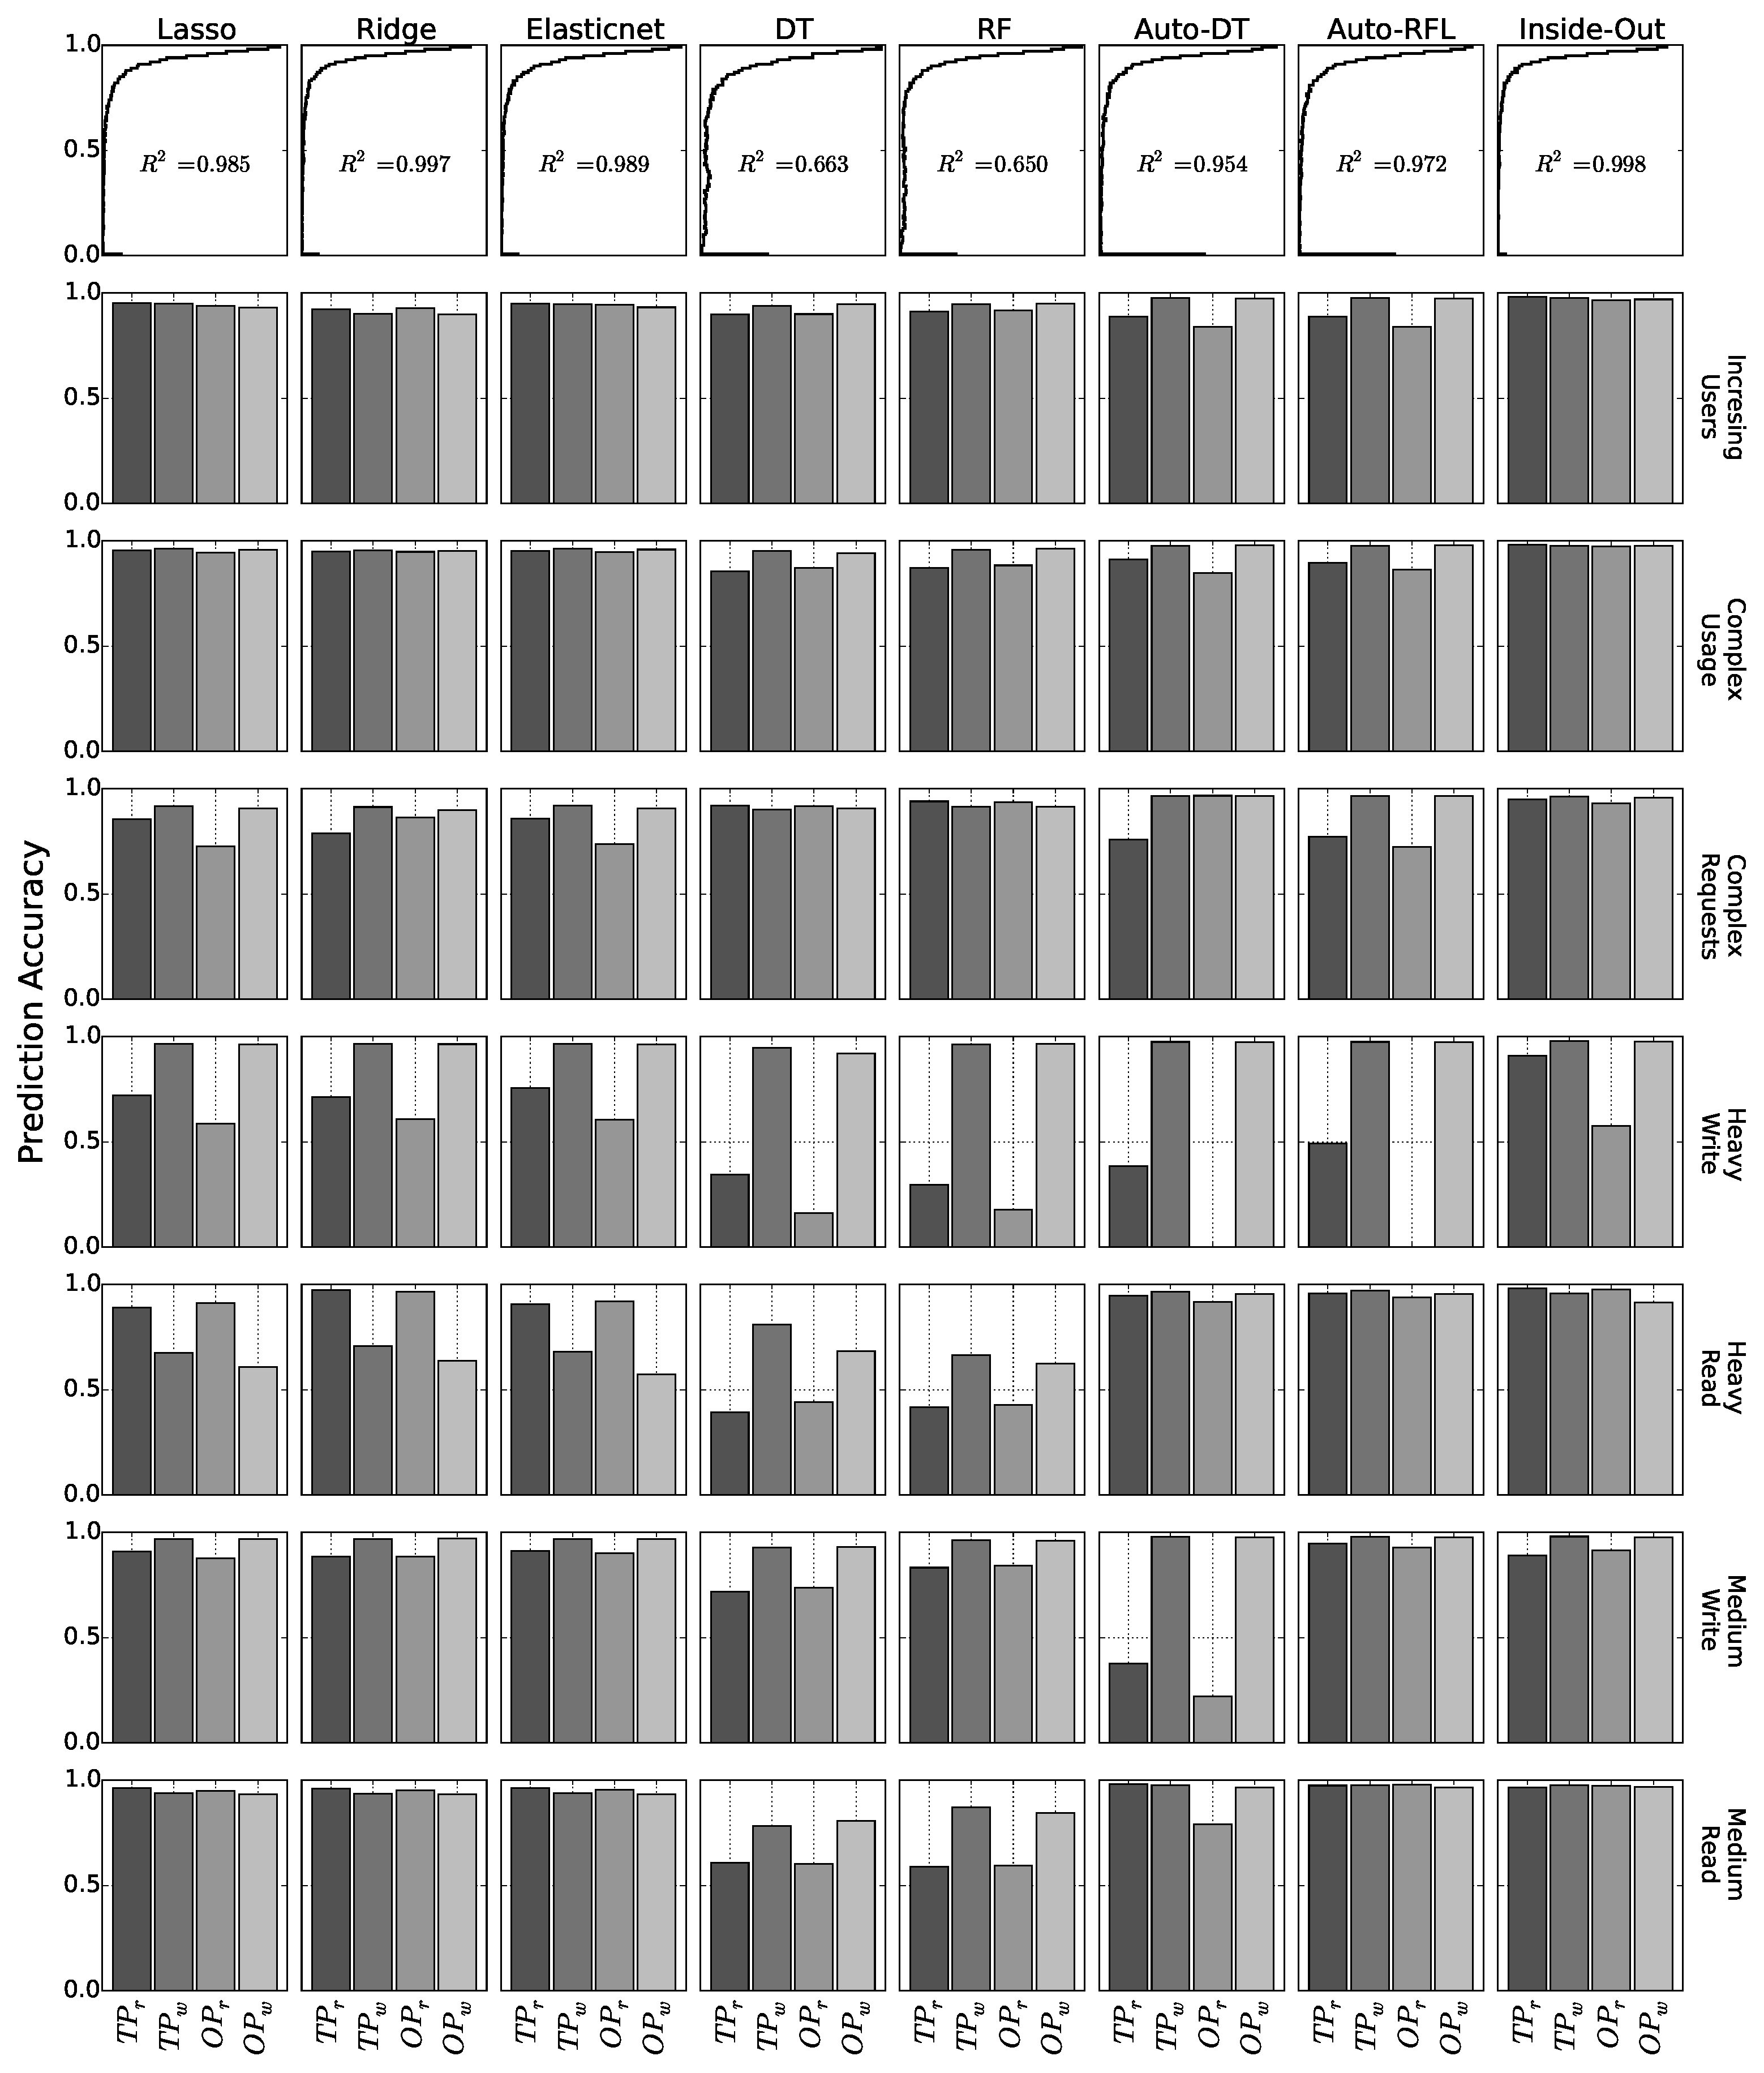
\includegraphics[width=0.9\textwidth]{Chapter-InsideOut/figures/unseen_workload_all_new.eps}
    \caption{Analysis of performance models with diverse workloads. Each bar is the average prediction accuracy. The top row is the probability density function of prediction accuracy for each performance model.}
    \label{fig:changing_workload}
\end{figure}

%\hfill\break

An SDS application needs to handle various request volumes, object/file sizes and different ratios of read/write workloads.
%In practice, it is difficult to obtain a training dataset that includes all access patterns.
First we examine whether Inside-Out can achieve accurate and consistent predictions when workload changes.


\paragraph*{Changing user behavior}
%\textbf{Changing user behavior.}

We increase the number of concurrent clients to stress the Ceph cluster.
%We push the Ceph cluster to a certain limit by increasing the parallelism of clients.
The \emph{\MakeLowercase{\scenarioMU}} scenario changes the number of COSBench clients and the \emph{\MakeLowercase{\scenarioCUB}} scenario increases the worker threads of each client.
As shown in \myfigure{\ref{fig:changing_workload}}, all prediction models perform well. The linear regression technique performs slightly better than the tree-based learning.
The linearly increasing load is well captured by linear models because of proportional change in low-level metrics.
When we switch to the \emph{\MakeLowercase{\scenarioCRB}} scenario, the variable request size slightly changes the behavior of Ceph, affecting prefetching and caching. 
We observe that the linear regression methods (Lasso, Ridge and Elastic Net) show drops in accuracy, e.g. 20\% in the $OP_r$ case; however, Inside-Out 
maintains good accuracy. 
The tree-based learning shows comparable predictions (5-10\% lower) with Inside-Out in these settings.



%\textbf{Complex request behavior.}
%Next, we change the workload from a constant IO request size to variable size.
%In this case, Inside-Out slightly improves the prediction accuracy over Lasso, %and outperforms the three linear models.
%Auto-DT and Auto-RFL show inconsistent prediction result with about 15\% %degradation of accuracy, comparing with the best case.
%One possible expalantion is that some important features filtered by DT and RF 
%are removed.
%Lasso and Elastic Net encounters accuracy drop in the read IOPS prediction


\paragraph*{Varying I/O pattern}

%The workload is a strong performance factor to a storage system \cite{Noorshams2013}.
%The read performance, for example, is affected by the amount of concurrent read or write operations.
Next, we consider workloads with different ratios of read to write operations.
\myfigure{\ref{fig:changing_workload}} shows that varying workload poses a big challenge to performance models. 
The linear regression methods (Lasso, Ridge and Elastic Net) present better prediction accuracy than tree-based models (DT, RL).
In addition, we observe that several models make poor predictions of $TP_r$ and $TP_r$.
The reason is that read behavior is largely affected by \textit{cache}, and large read variance contributes to low prediction accuracy.
Inside-Out performs consistently well, whereas the three linear regression techniques show accuracy drops.
One exception is the $OP_r$ prediction in the \textit{write-intensive} scenario even though $TP_r$ prediction is accurate.
As we will show later in Section~\ref{sec:online_learning}, \emph{over- and under-predictions} cause such behavior. 
The self-learning property of Inside-Out improves its prediction accuracy as it keeps learning the new storage behavior.


\begin{figure}
    \centering
    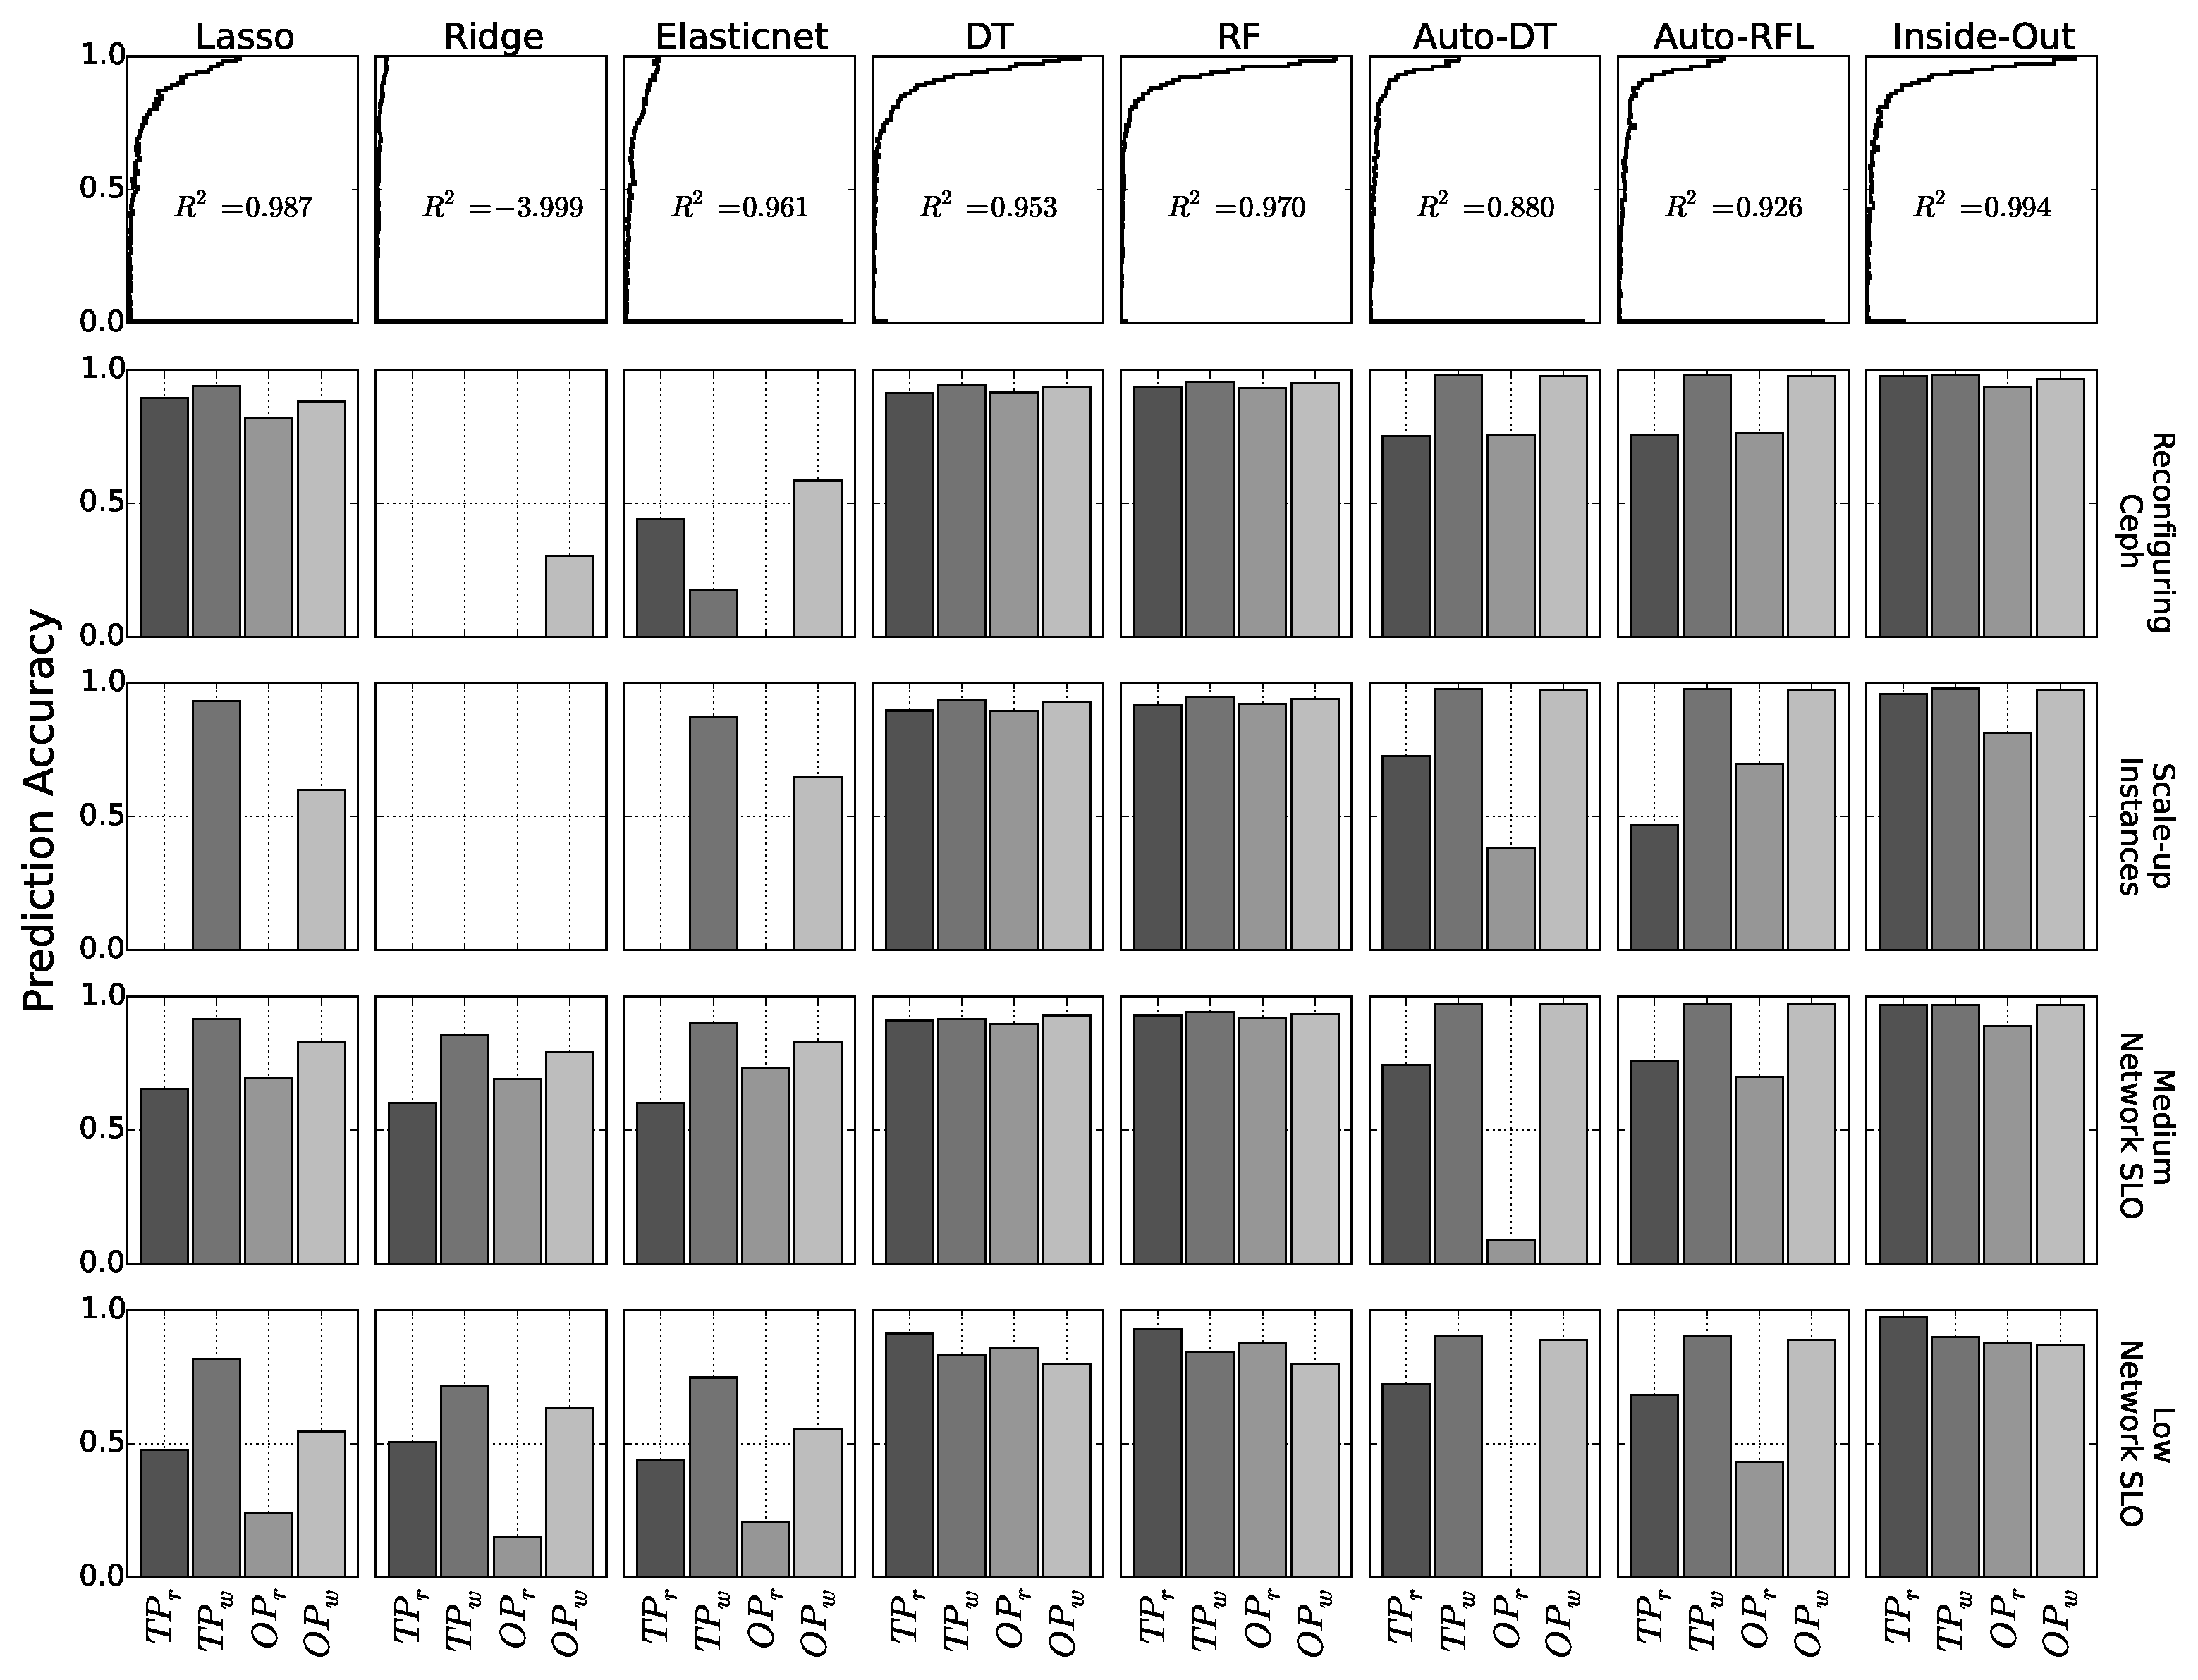
\includegraphics[width=0.9\textwidth]{Chapter-InsideOut/figures/unseen_configuration_all_new.eps}
    \caption{Comparison of performance models when the storage service is reconfigured: Ceph, VMs and network SLOs}
    \label{fig:reconfiguring_storage}
\end{figure}


\paragraph*{Summary}
The linear regression models achieve high prediction accuracy, great goodness-of-fit ($>0.98$) and consistency in prediction 
for many instances (see the distribution of prediction accuracy in \myfigure{\ref{fig:changing_workload}}), but they 
are not consistent across all prediction scenarios.
Inside-Out achieves good prediction accuracy across all cases consistently because the two-level approach 
filters out many irrelevant features in the first step, thereby presenting a smaller relevant feature space to the second step. 
The tree-based learning methods (DT and RF) do not show consistent prediction across all scenarios.
Auto-DT and Auto-RFL, which use DT and RF as the filter algorithms, are not as consistent as Inside-Out.

\vspace{1ex}

%\subsubsection{Reconfiguring Storage}
\subsubsection{Can Inside-Out handle different system configurations?}
\label{sec:unseen_configuration}

We study whether low-level metrics can capture the storage behavior when it is reconfigured by tenants. The results are reported in \myfigure{\ref{fig:reconfiguring_storage}}.


\textbf{Reconfiguring Ceph.}
The first change is to add one extra Ceph monitor daemon. %\chin{which increases the capability to handle a large number of clients.}
Ridge and Elastic Net fail to generate consistent predictions, but Lasso is able to achieve around 80\% to 90\% prediction accuracy.
DT, RF and Inside-Out have very close prediction accuracies, but Auto-DRL and Auto-RFL perform slightly worse in predicting $TP_r$ and $OP_r$.

\textbf{Scale-up instances.}
Increasing CPU and memory allocation to Ceph VM instances improves Ceph's ability to handle more requests.
In this test, we change the instance type from m1.small (1 vCPU, 2GB memory) to m1.medium (2 vCPUs, 4GB memory).
The linear models are unable to predict $TP_r$ and $OP_r$, but Inside-Out's two-level learning performs well by avoiding the overfitting problem. 

\textbf{Network SLOs.}
Here we consider the case where the amount of network bandwidth allocated to Ceph VMs is limited. 
We use Linux network throttling tool \textit{tc} to limit network bandwidth at 500 Mbps and 250 Mbps for medium and low bandwidth SLOs, respectively.
We observe that linear models without the two-level method do not show comparable prediction accuracy across both throughput and IOPS predictions.
The tree-based learning models, on the other hand, achieve 80\% to 90\% accuracy, comparable to Inside-Out.


\textbf{Summary.}
Tree-based learning (DT, RF) models demonstrate promising prediction in terms of prediction accuracy and consistency.
Lasso, Ridge and Elastic Net show inconsistent behavior in the above four scenarios.
Inside-Out, on the other hand, provides consistent predictions and improves Lasso, from 23.9\% to 87.6\% in the extreme case.


\begin{figure}
    \centering
    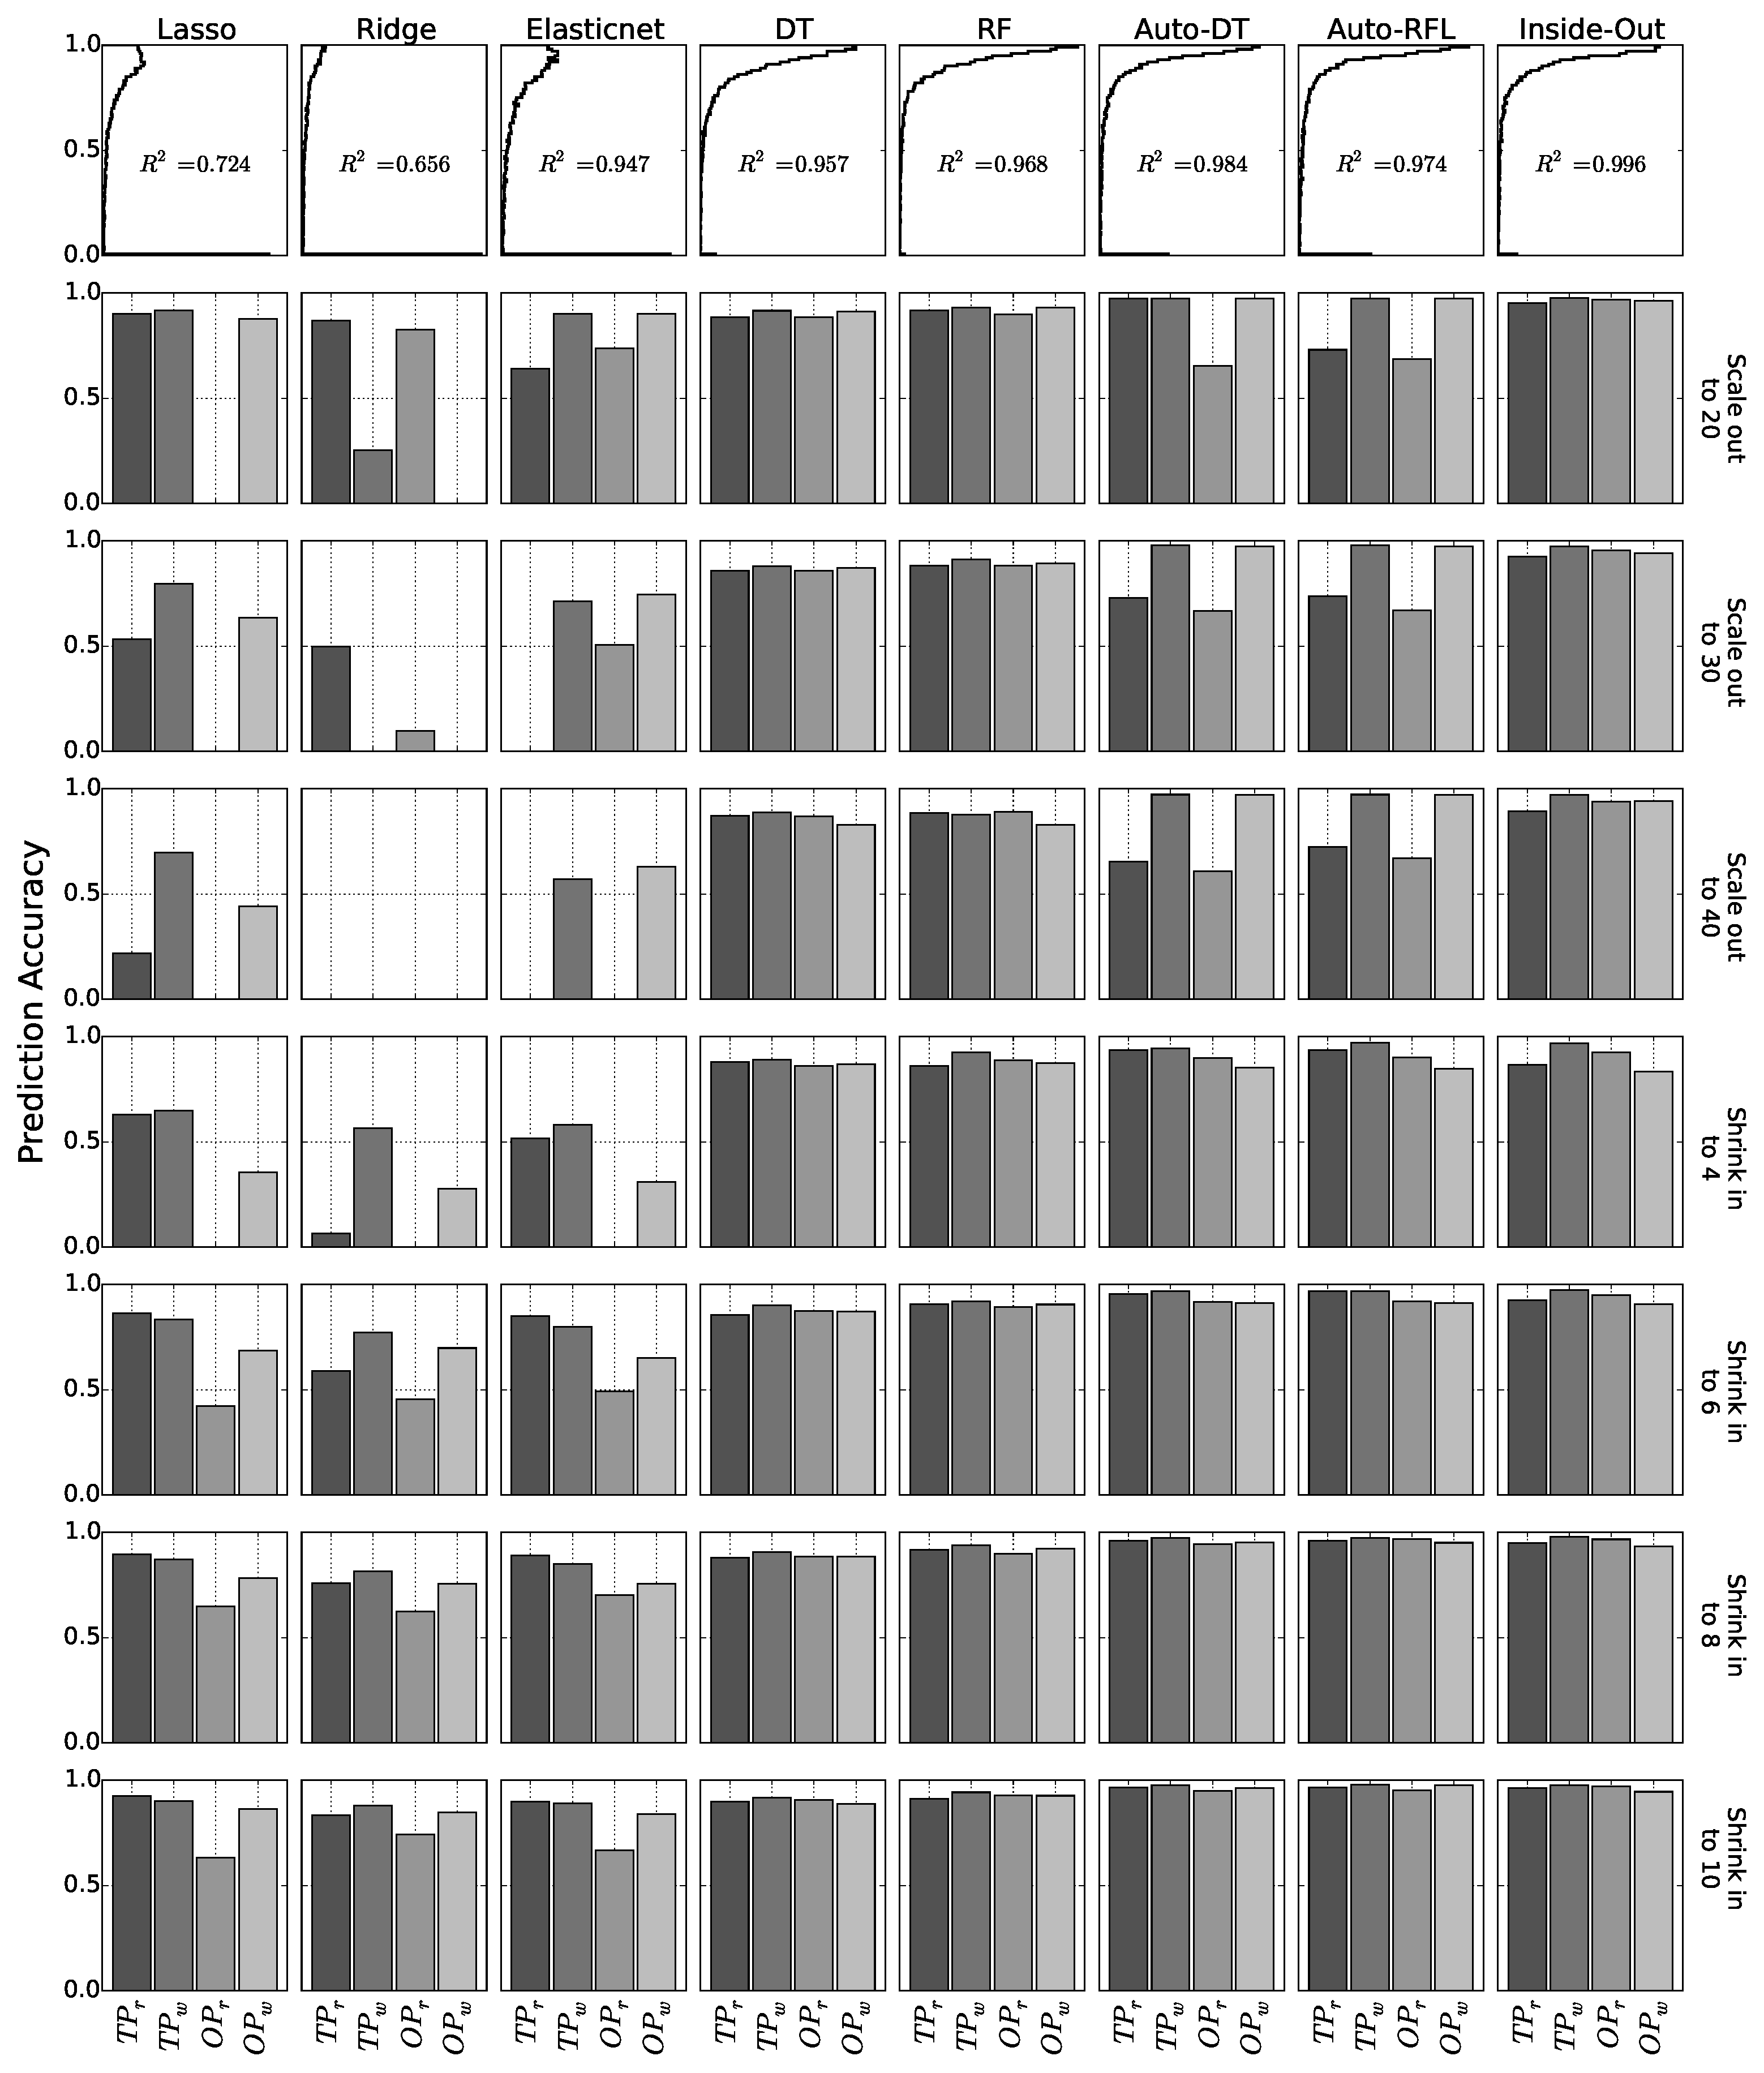
\includegraphics[width=0.9\textwidth]{Chapter-InsideOut/figures/unseen_scale_all_new.eps}
    \caption{Comparison of model performance in the on-demand scaling scenario. In the scale-out scenario, a performance model trained with 10 Ceph nodes is used to predict the performance of Ceph cluster with 20, 30 and 40 nodes.}
    \label{fig:elasticity}
\end{figure}


\subsection{Prediction Performance in a Multi-tenant Cloud}

This section examines the modeling performance of Inside-Out.
We first evaluate whether Inside-Out is able to extrapolate
performance of a larger Ceph cluster. 
Next, we evaluate how Inside-Out performs
when systems are subject to performance interference.

\subsubsection{Elastic Storage (On-demand Scaling)}
\label{sec:scaleout_prediction}

A storage service needs to grow or shrink its capacity on demand.
We evaluate Inside-Out's ability to capture the storage behavior at different system scales.
As shown in \myfigure{\ref{fig:elasticity}}, we use training data collected from 
4, 6, 8, and 10 nodes, and then predict the performance of 20, 30, and 40 nodes.
We also evaluate prediction accuracy in the \emph{shrink-in} scenario.
For both read and write throughput predictions, the linear models exhibit high variance.
In the $OP_r$ and $OP_w$ cases, the prediction results are not even comparable to the other methods.
Inside-Out, on the other hand, helps mitigate this issue, and achieves more than 90\% accuracy.
With increasing sizes of the storage, the prediction accuracy decreases because the prediction target 
becomes increasingly different from the training data.
Running a benchmark test against a very large system is time-consuming.
Here we demonstrate that Inside-Out can predict performance for systems that are 
four times larger than the system for which training data was collected.
%Due to resource limitations, we cannot show the upper bound of the largest system size that we can predict.
%However, we believe the upper bound can increase as the performance model keeps learning the system behavior.

\begin{figure}
    \centering
    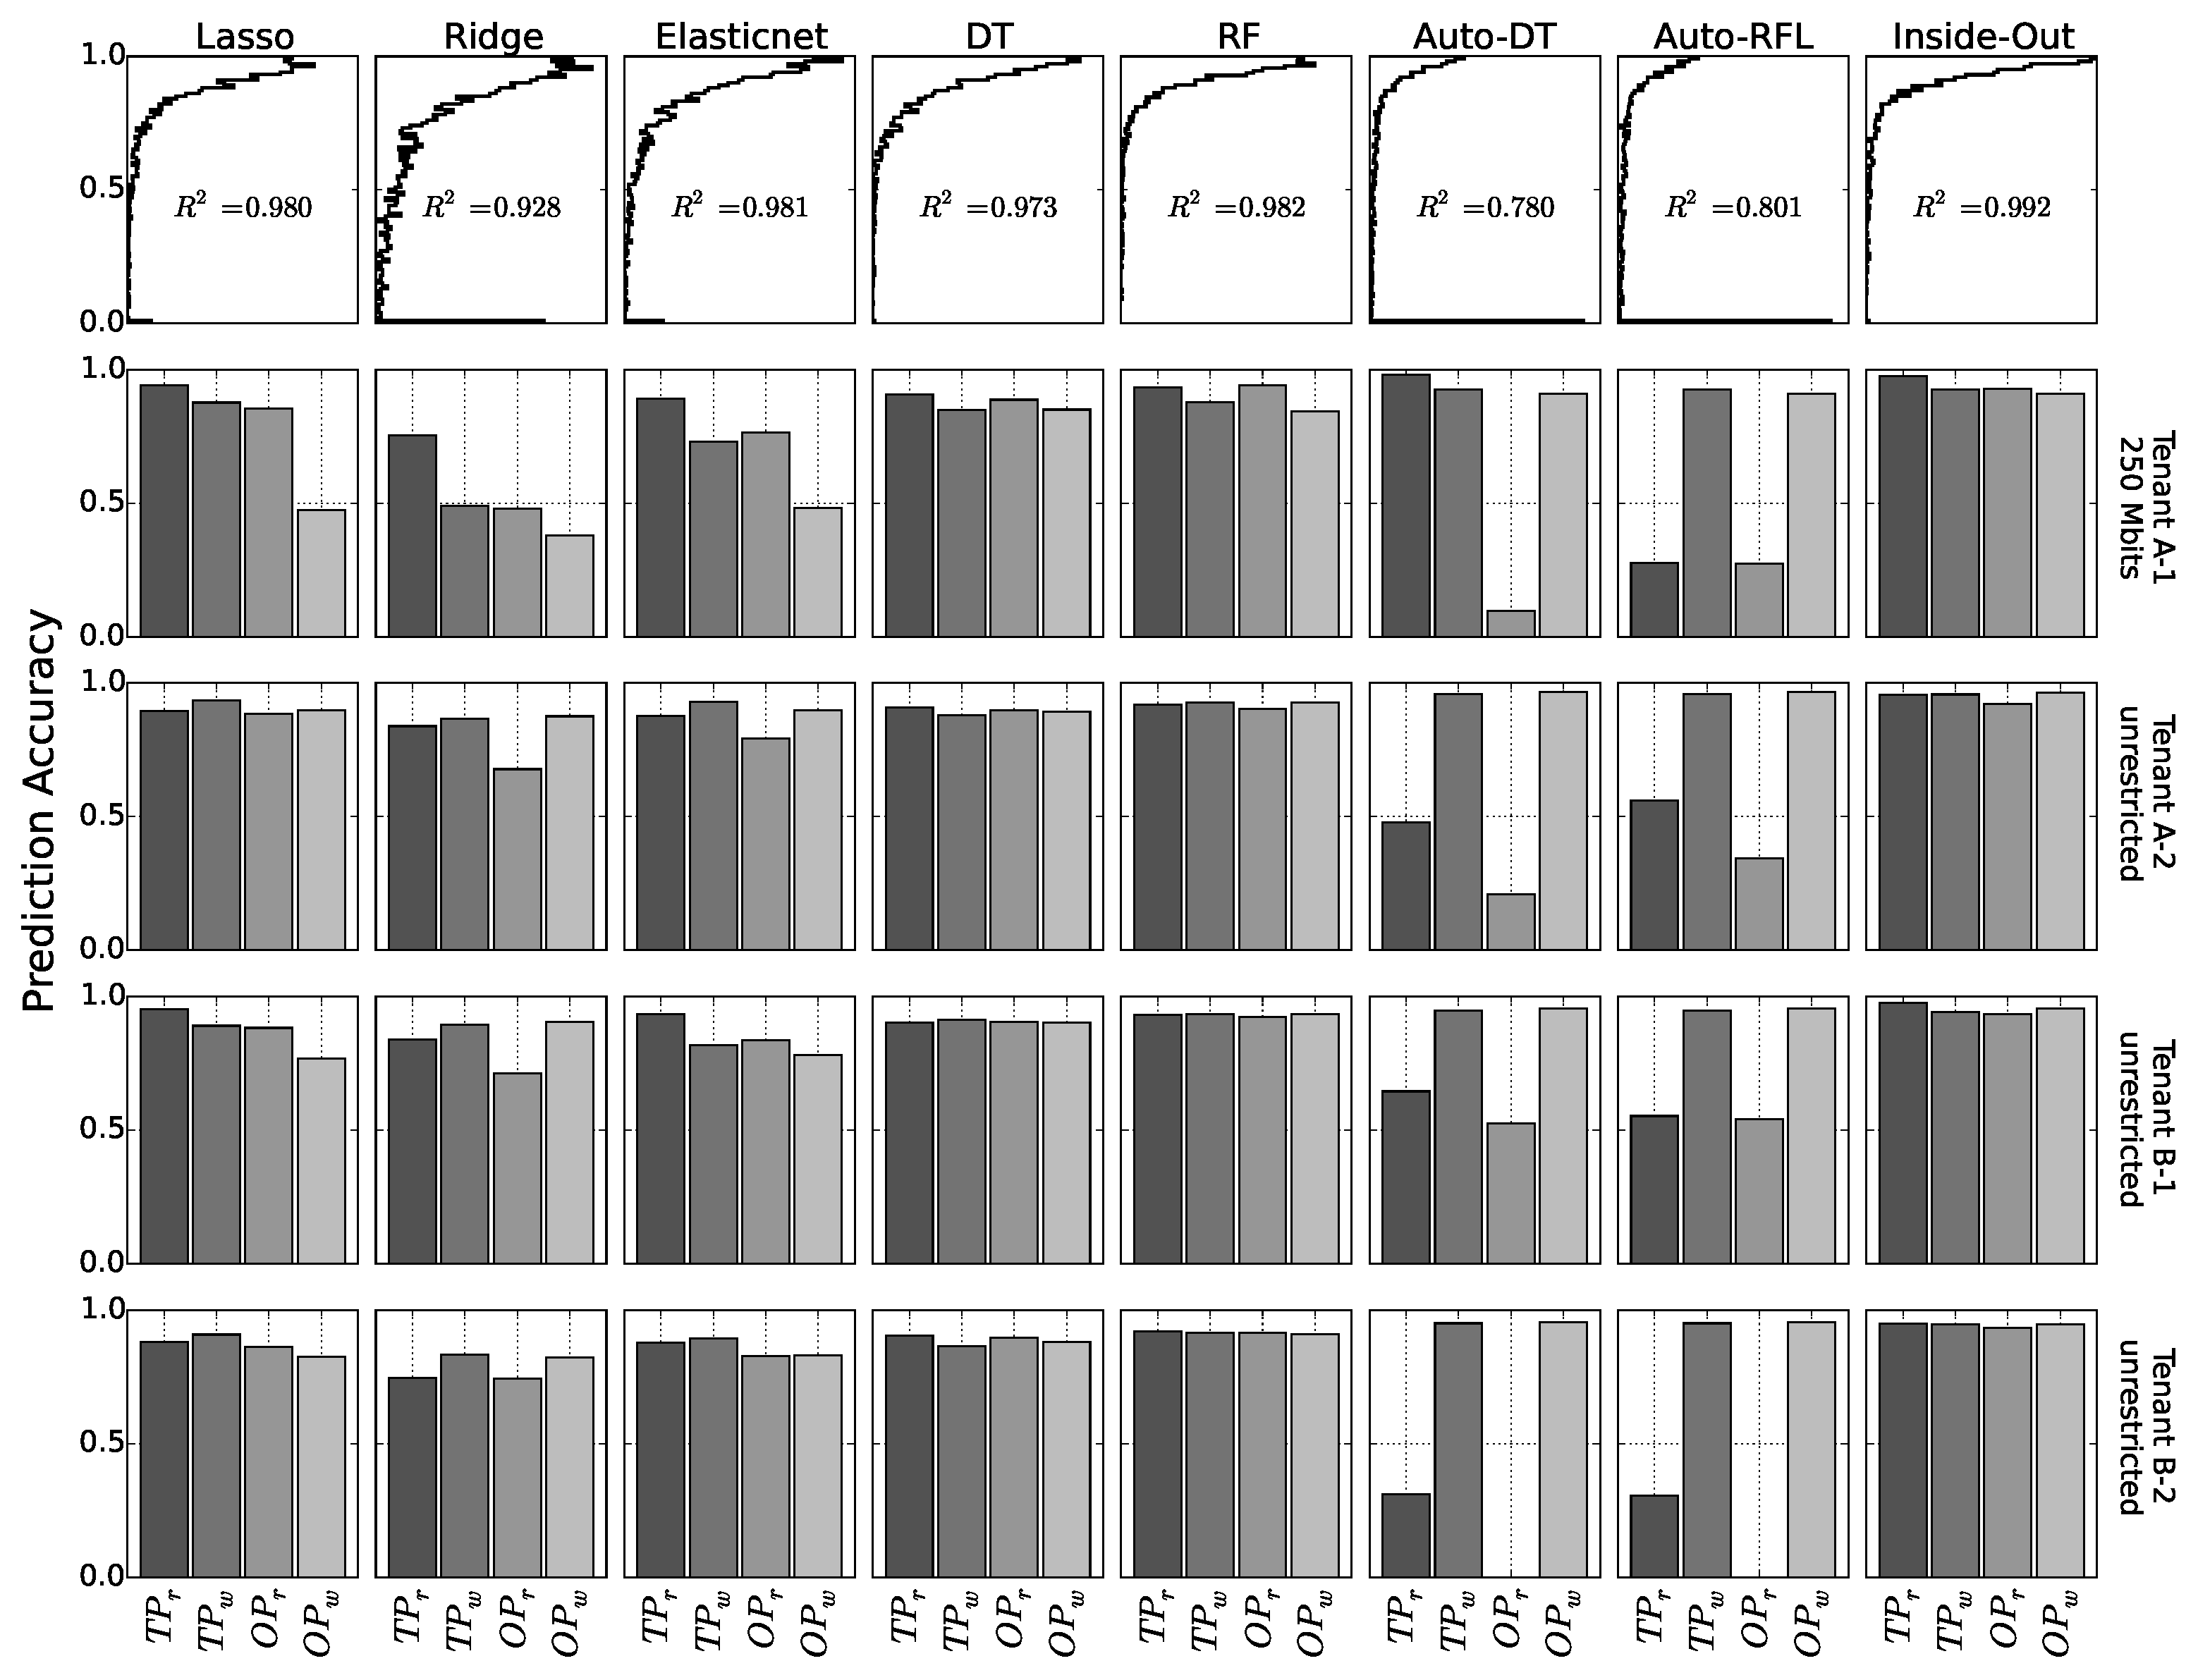
\includegraphics[width=0.9\textwidth]{Chapter-InsideOut/figures/multi_tenancy_all_new.eps}
    \caption{Prediction accuracy in a multi-tenancy scenario. Tenant A-1 is co-located with Tenant B-2. Tenant A-1 is throttled at 250Mbps. Tenant B-1 and B-2 are co-located without any traffic throttling.}
    \label{fig:multi_tenancy}
\end{figure}


\begin{figure*}
    \centering
    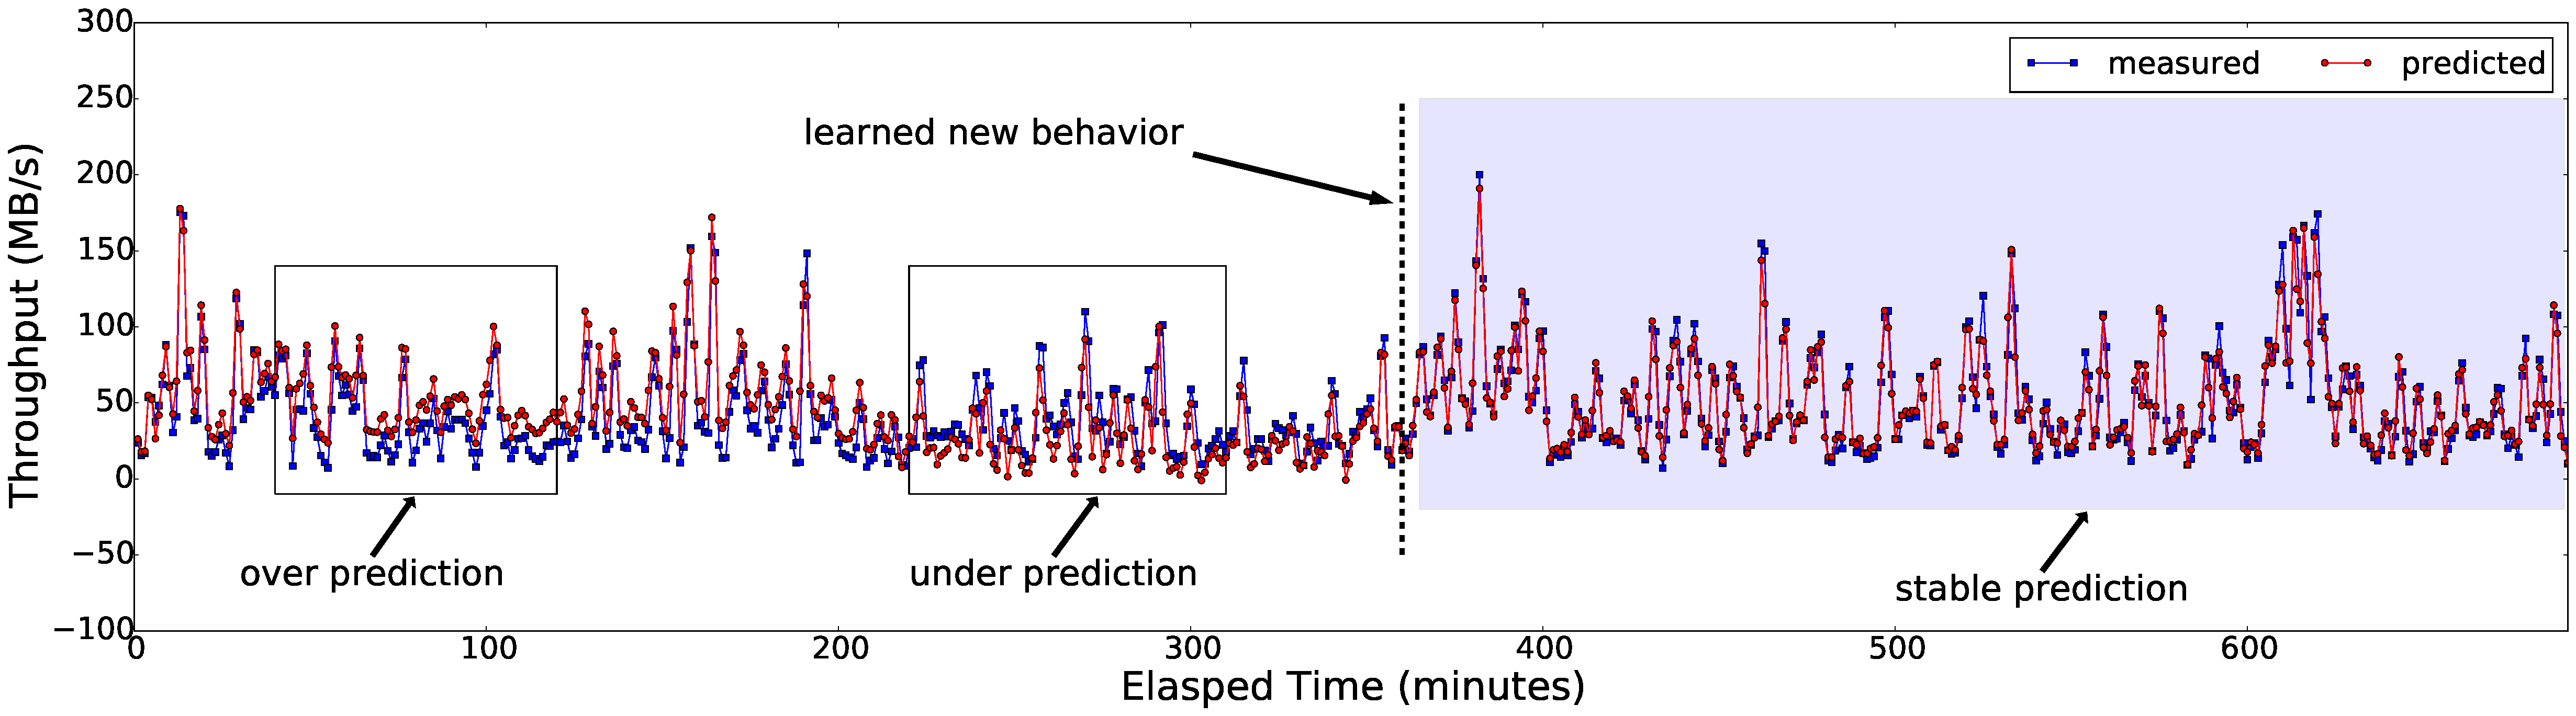
\includegraphics[width=0.9\textwidth]{Chapter-InsideOut/figures/real-world_tp_read.pdf}
    \caption{Application of Inside-Out to real time prediction of read throughput on a 10-node Ceph cluster.  Inside-Out starts from a simple prediction model trained by our collected benchmarking data.  Inside-Out keeps learning the storage behavior while improving prediction accuracy over time.}
    \label{fig:real_workload}
\end{figure*}


\subsubsection{Multi-Tenancy}
 
Next we evaluate Inside-Out's ability to adapt to performance interference among storage tenants.
We consider two cases for this evaluation. 
Each tenant runs a Ceph cluster with 10 OSDs separately, but tenants share the same 10 physical machines.
In the first case, we restrict the bandwidth of only the first tenant at 250Mbps.
%Two tenants compete for resources and \chin{\textbf{Tenant A-1}} has lower bandwidth SLO.
In the second case, we run two concurrent Ceph clusters but without network throttling.
\myfigure{\ref{fig:multi_tenancy}} shows that most prediction models are able to achieve more than 80\% accuracy.
The linear models like Ridge and Elasticnet yield lower prediction accuracies in some cases; however, Inside-Out performs well consistently.
Performance interference is challenging for a performance model designed for an isolated environment.
This evaluation demonstrates that the low-level performance metrics are good proxies for measuring
the end-to-end storage performance, even in a shared SDS environment.
%These metrics are able to reflect the behavior changes in the storage system.

%low-level performance feature selection approach is effective in capturing end-to-end performance, even under high storage interference.
%This property is important to SDS because it can help guarantee reliable end-to-end performance in a shared SDS environment.



\begin{comment}
\begin{figure*}
    \centering
    \includegraphics[width=0.9\textwidth]{figures/synthetic.eps}
    \caption{An online prediction scenario about six-hour long workload.  This synthetic workload is composed of 360 stages and each stage uniformly selects parameters such as workload types, request sizes and the number of clients.  The average stage duration is 60 seconds with standard deviation 20 seconds.}
\end{figure*}
\end{comment}

\begin{comment}
\begin{figure*}
    \centering
    \begin{subfigure}[b]{0.45\textwidth}
        \includegraphics[width=\textwidth]{figures/synthetic_read.eps}
        \caption{Read Throughput}
        \label{fig:synthetic_read}
    \end{subfigure}
    ~ %add desired spacing between images, e. g. ~, \quad, \qquad, \hfill etc.
      %(or a blank line to force the subfigure onto a new line)
    \begin{subfigure}[b]{0.45\textwidth}
        \includegraphics[width=\textwidth]{figures/synthetic_write.eps}
        \caption{Write Throughput}
        \label{fig:synthetic_write}
    \end{subfigure}
    \caption{An online prediction scenario about six-hour long workload.  This synthetic workload is composed of 360 stages and each stage uniformly selects parameters such as workload types, request sizes and the number of clients.  The average stage duration is 60 seconds with standard deviation 20 seconds.}
    \label{fig:synthetic_workload}
\end{figure*}
\end{comment}

%\subsection{Synthetic Workload}
\subsection{Online Self-Learning}
\label{sec:online_learning}

%Our goal is to apply Inside-Out to an online system so that SDS providers can guarantee the performance of a storage service hosted on their SDS platform.
%To evaluate this potential, 
Next, we create several synthetic workloads with mixed read/write ratios.
This synthetic workload spans 12 hours with 720 stages.
Each stage is 60-second long on average, with a standard deviation of 20 seconds.
We run four COSBench virtual machines for benchmarking and up to eight threads per COSBench client, with 10 Ceph OSDs and one monitor daemon.
We use Inside-Out to build an initial performance model with the training dataset described in Section~\ref{sec:dataset}.
\myfigure{\ref{fig:real_workload}} shows the prediction result for read throughput.
We can observe that the generated model can capture the overall trend, but suffers from over and under predictions.
This is because our training dataset is generated from a relatively clean environment, \ie the OS memory is flushed before any benchmarking process.
However, in the online prediction setting, cache is continuously consumed by non-stop client requests, which 
causes the real time storage behavior to be different from the training dataset.
With continuous monitoring of the performance of the storage service, 
we use Inside-Out to generate a new performance model at the sixth hour.
\myfigure{\ref{fig:real_workload}} shows that Inside-Out learns the new storage behavior and therefore, 
the over- and under-prediction issues are greatly mitigated.
%This evaluation demonstrates the potential of Inside-Out when applying it in an online system.
By continuously learning the storage behavior, SDS can accurately capture performance changes and therefore is able to provide reliable storage service.

%the problems due to over- and under-predictions are greatly mitigated.
%This evaluation demonstrates how Inside-Out can be used to continuously learn the storage behavior in an online system.


\begin{figure}
\centering
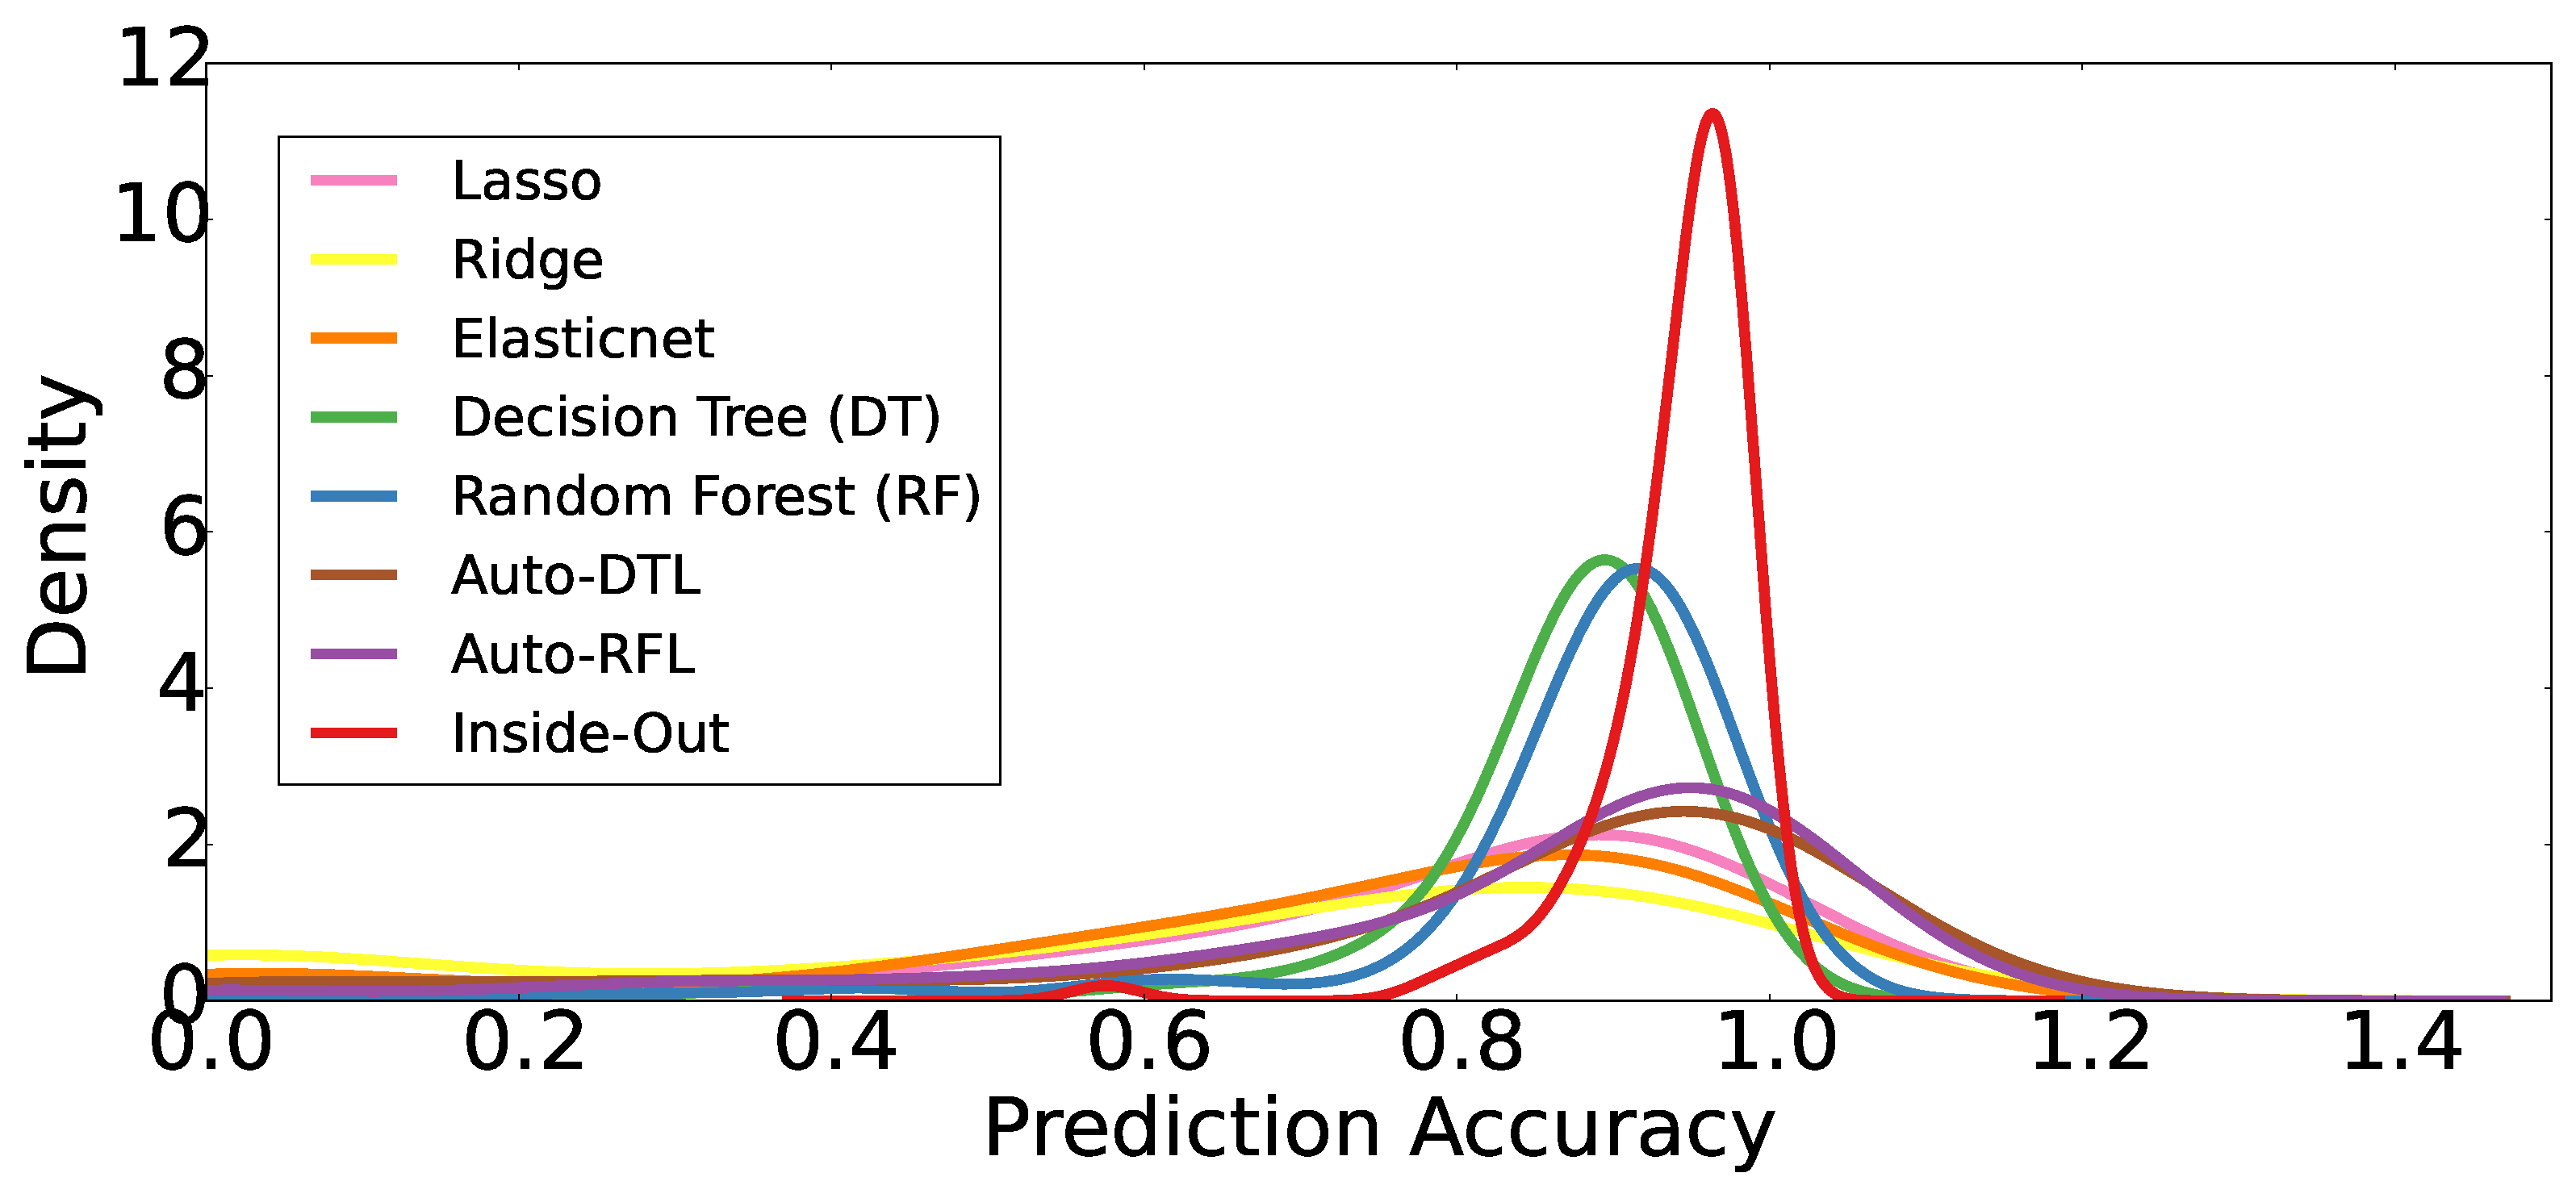
\includegraphics[width=0.9\textwidth, keepaspectratio]{Chapter-InsideOut/figures/aggregate_median.eps}
\caption{Kernel density function of prediction accuracy from \myfigure{\ref{fig:changing_workload}} to \myfigure{\ref{fig:multi_tenancy}}.  Each colored line represents the density function of a modeling approach.  Inside-Out is more consistent and accurate across almost every prediction case.}
\label{fig:aggregate}
\end{figure}


\vspace{1ex}
\subsection{Discussion}
We have shown that low-level performance metrics are useful to predict end-to-end throughput and IOPS.
%We applied Inside-Out to latency prediction and observe large variance and inconsistency.
%\chin{One} possible explanation is insufficient features and high variance in latency.
%The \chin{collected} low-level metrics are related to utilization, and these metrics might not provide enough information to fit a good model for predicting latency.
%Common approaches usually require request-level information \cite{Wang2004}.
%We need to further investigate latency prediction with other alternative generic low-level performance metrics.
Our evaluation has shown that low-level performance metrics are good indicators of end-to-end throughput and IOPS. 
Most existing performance models exhibit an inconsistent prediction behavior in the presence of diverse storage scenarios, 
such as changing workload, storage reconfigurations,
growing/shrinking storage, and multi-tenancy environments.
Our proposed two-level learning method can greatly improve prediction accuracy and yield consistent behavior.
Machine learning provides powerful tools, but they need to be used intelligently to achieve the best prediction accuracy. 
\myfigure{\ref{fig:aggregate}} shows the kernel density function of prediction accuracy across all prediction scenarios.
Inside-Out is a clear winner in terms of accuracy and consistency. 
More importantly, Inside-Out is able to learn new storage behavior, thereby enabling the performance model to adapt to the complex SDS environment.





\section{Discussion}
\label{sec:discussion}


\subsection*{Tuning Searching Performance}

\scout uses ``probability threshold'' and ``misprediction tolerance'' as stopping criteria.
%We examine how they affect the search performance of \scout.\\

\subsubsection*{Probability Threshold}
\scout chooses the next configuration to evaluate
based on the probability of improvement and
stops when the probability is lower than the probability threshold $\alpha$.
\myfigure{\ref{fig:single_probability_threshold}} shows that
a higher probability threshold is pessimistic and 
terminates the search process prematurely,
hence, shorter search path
and unstable search results). 
The probability threshold presents a trade-off between
search performance and search cost.
The right threshold must consider
the reliability curve of classification methods~\cite{niculescu2005predicting}.

\subsubsection*{Misprediction Tolerance}
\scout terminates the search process if the selected configurations do not improve the current best choice (considered as a misprediction).
\scout maintains a counter of mispredictions.
A higher limit tolerates more mispredictions but yields better search performance due to more chances.
A proper limit should consider both
the size of search space and the accuracy of prediction.
In \myfigure{\ref{fig:single_misprediction_tolerance}},
we show that a higher tolerance level leads to better search performance but higher search cost.
This trade-off is similar to the probability threshold.

\begin{figure}[!htbp]
\centering
\begin{subfigure}[b]{0.4\textwidth}
    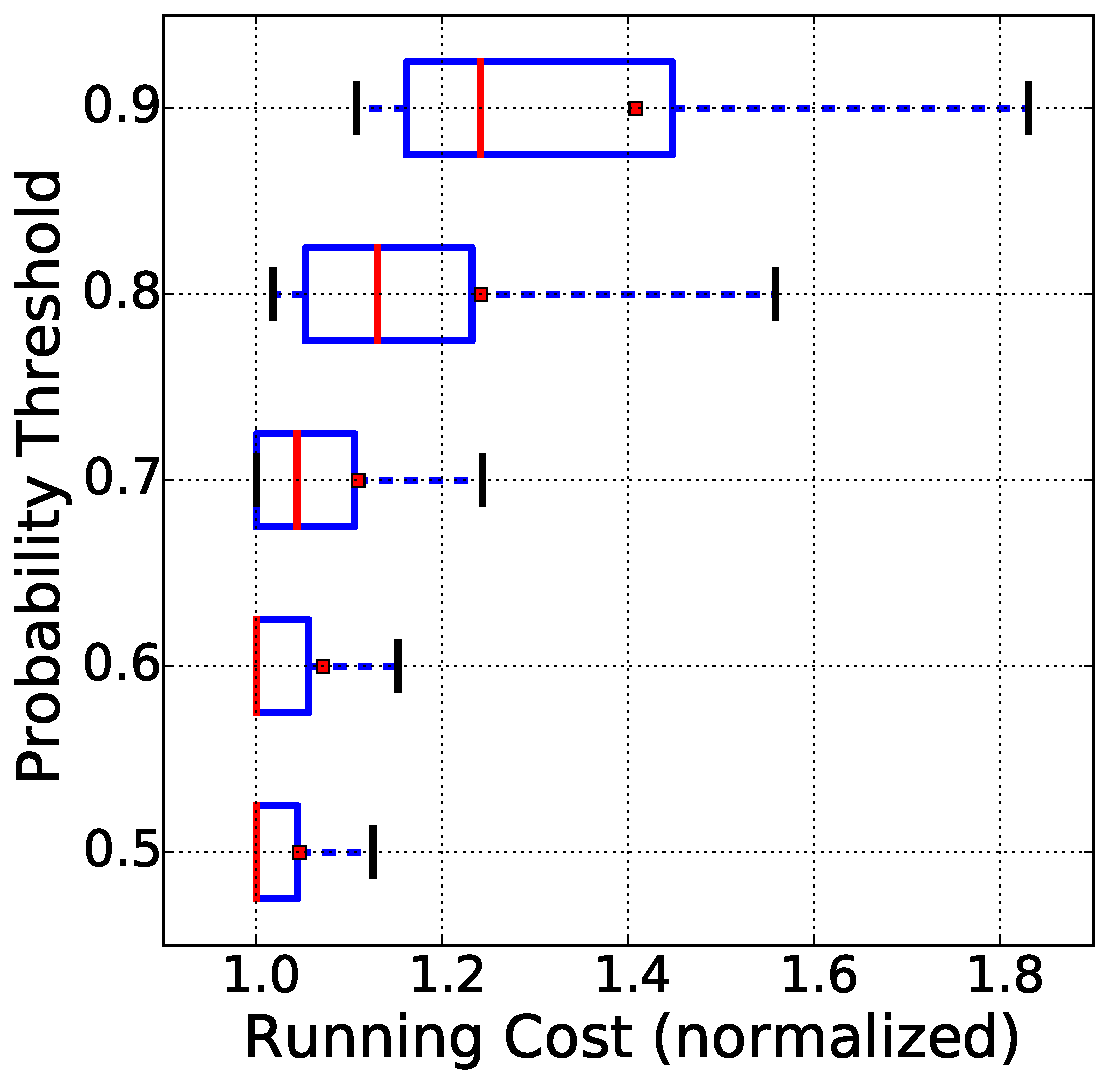
\includegraphics[width=\linewidth]{figures/single_cost_tuning_probability_performance.pdf}
    \caption{Search Performance}
    \label{fig:single_cost_tuning_threshold_performance}
\end{subfigure}
\begin{subfigure}[b]{0.4\textwidth}
    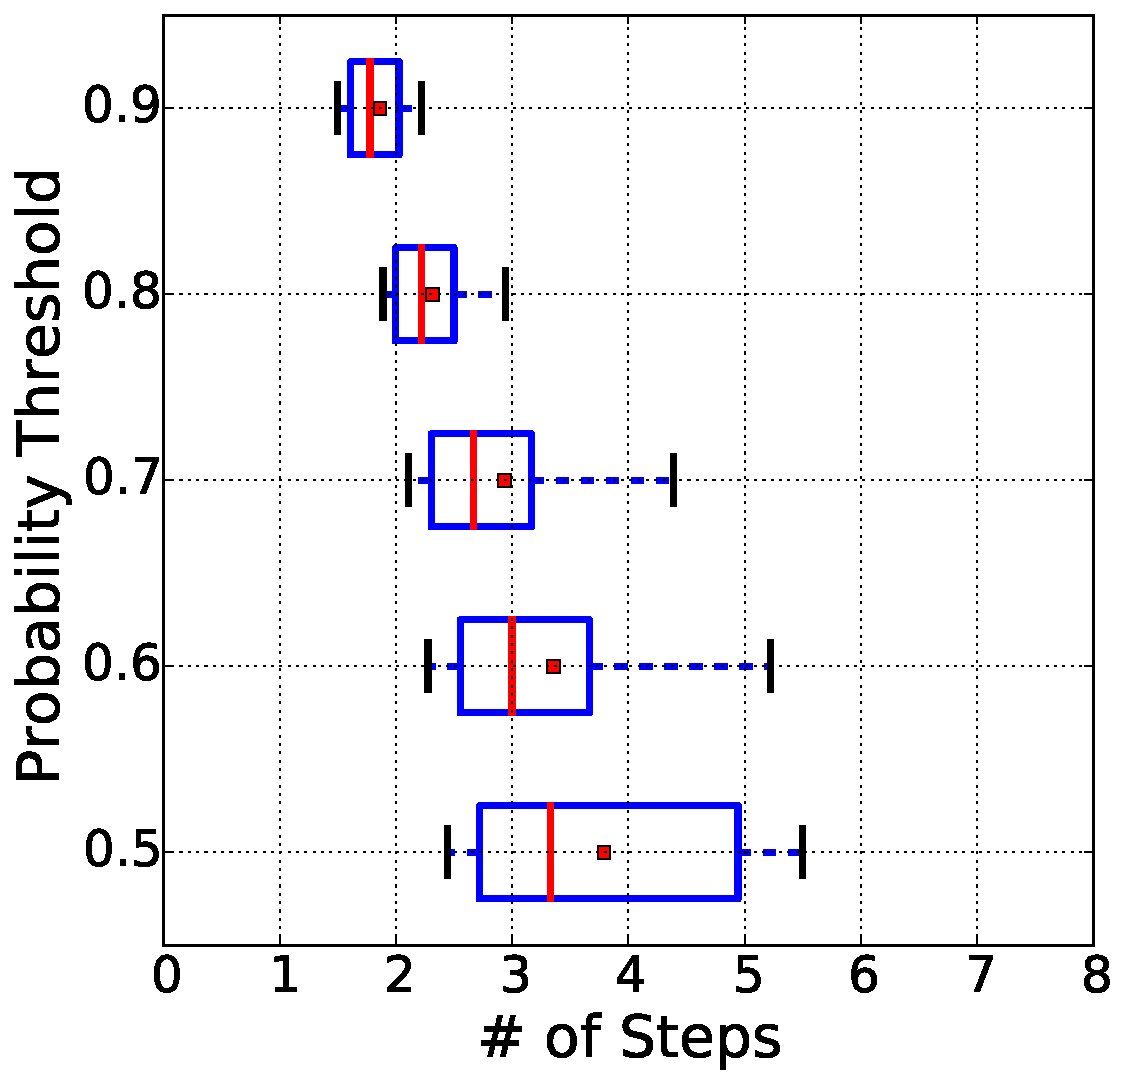
\includegraphics[width=\linewidth]{figures/single_cost_tuning_probability_steps.pdf}
    \caption{Search Cost}
    \label{fig:single_cost_tuning_threshold_steps}
\end{subfigure}
\caption{\small{\textbf{Tuning the probability threshold.} A smaller threshold generates a longer search path but ensures better search performance.}}
\label{fig:single_probability_threshold}
\end{figure}

\begin{figure}[!htbp]
\centering
\begin{subfigure}[b]{0.4\textwidth}
    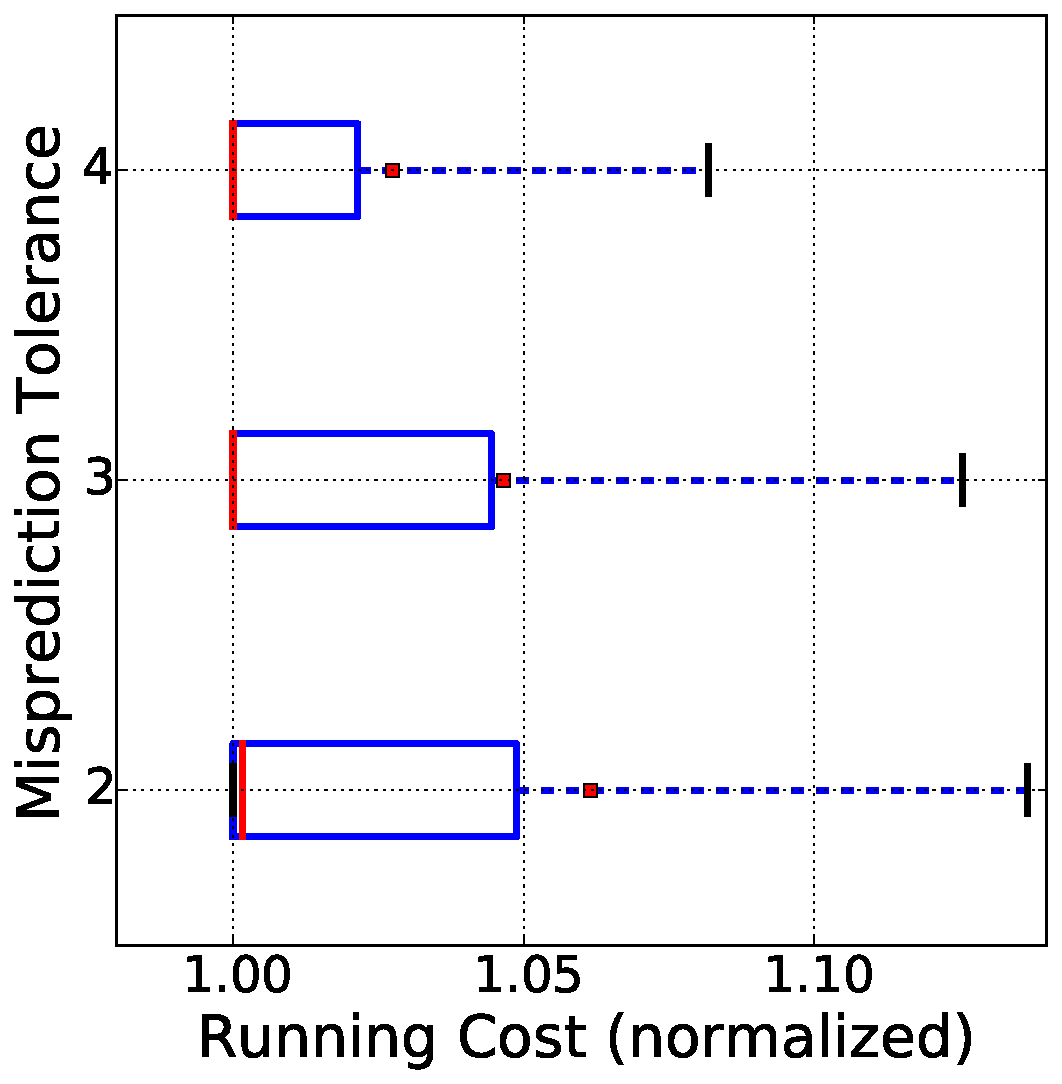
\includegraphics[width=\linewidth]{figures/single_cost_tuning_tolerance_performance.pdf}
    \caption{Search Performance}
    \label{fig:single_cost_tuning_tolerance_performance}
\end{subfigure}
\begin{subfigure}[b]{0.4\textwidth}
    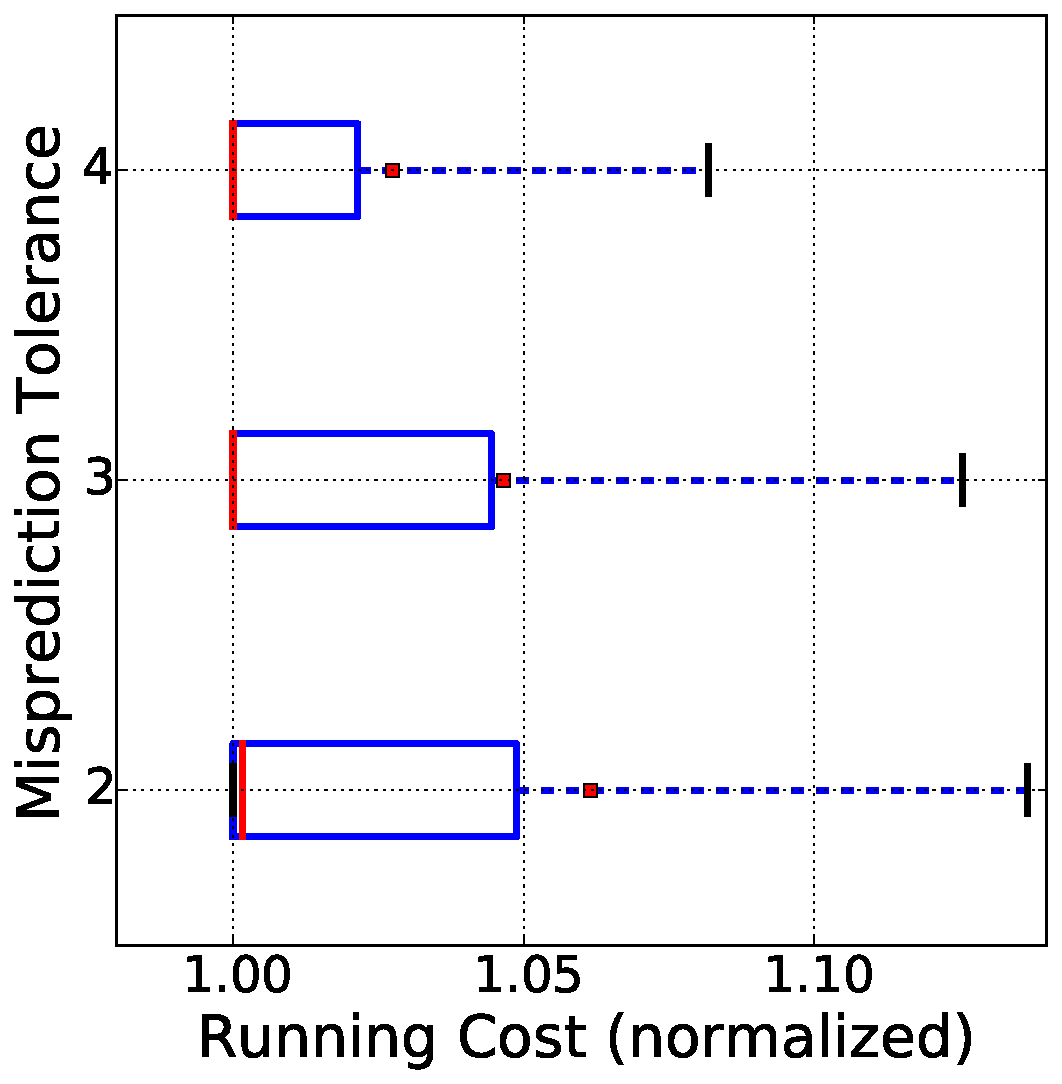
\includegraphics[width=\linewidth]{figures/single_cost_tuning_tolerance_performance.pdf}
    \caption{Search Cost}
    \label{fig:single_cost_tuning_tolerance_performance}
\end{subfigure}
\caption{\small{\textbf{Tuning the misprediction tolerance.} A higher tolerance to mispredictions generates higher search cost.}}
\label{fig:single_misprediction_tolerance}
\end{figure}


\subsection*{Alternative search strategies}
\scout generates the probability vector $P_{i}$
for each new observation (running the workload on $S_i$).
Our current search strategy only uses information from the latest observation.
\scout stores historical observations and therefore,
the next search step can be determined using several past observations.
%In \myfigure{\ref{fig:search_strategies}}, we illustrate a way to incorporate other observations.
Given two observations on $S_1$ and $S_2$ and two unevaluated configuration $S_3$ and $S_4$,
\scout generates prediction probability
$P_{13}$ and $P_{14}$ from $S_1$, and $P_{23}$ and $P_{24}$ from $S_2$.
Instead of choosing $P_{23}$ after the second step,
\scout should choose $P_{14}$ when $S_2$ is much worse than $S_1$ (due to mispredictions).
This strategy is more likely to avoid bad choices.
On the other hand, 
\scout currently relies on offline performance modeling.
Another alternative is to update the prediction model upon new observations.
For unseen workloads, this update enables \scout to improve prediction accuracy.
However, the downside is the cost of retraining the model.
An online learning method might help reduce the retraining cost.
The two possible alternatives remain as future work.

\begin{figure}[!htbp]
 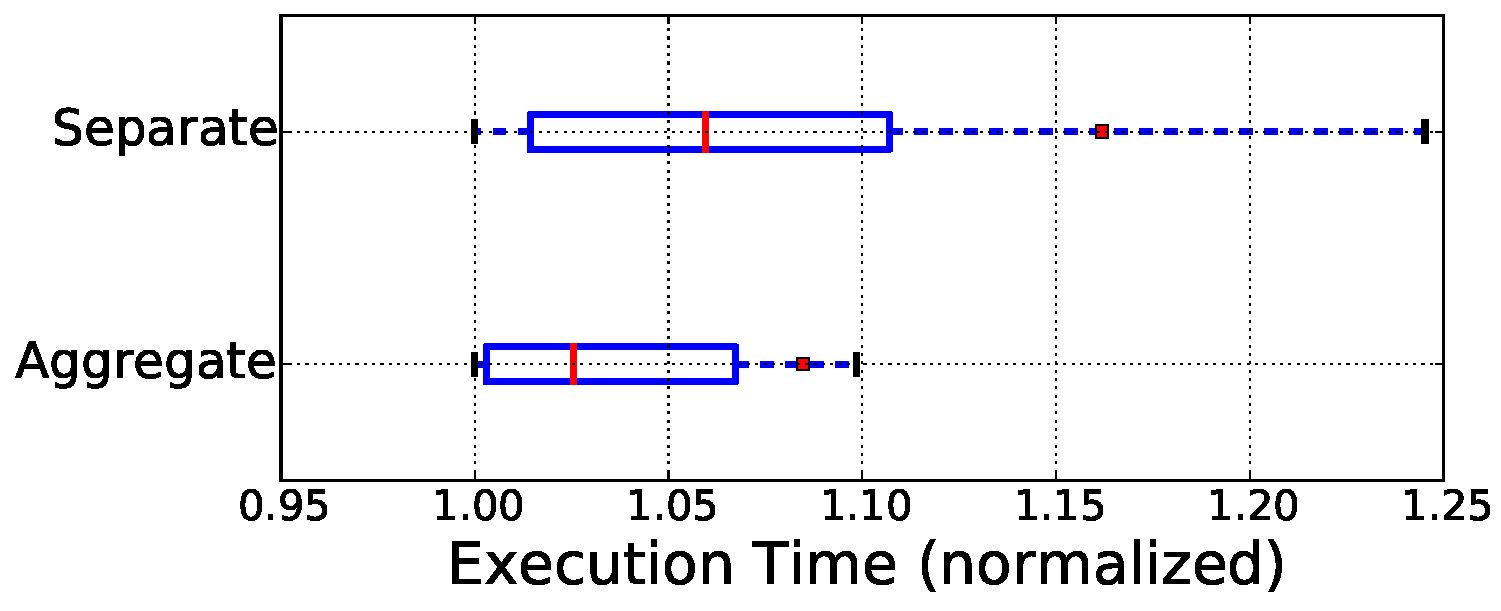
\includegraphics[width=.8\textwidth]{figures/multiple_size_of_dataset.pdf}
 \centering
 \caption{\textbf{Universal performance models.}
 Training data form multiple systems improves prediction.}
 \label{fig:prediction_accuracy_comparison}
\end{figure}

\textbf{Universal Prediction Models.}
% The performance models are built to find the best cloud configuration for a certain workload. These performance models generalize the information learned from the evaluated configurations. This helps the model to be accurate while predicting new cloud configurations. 
In prior work, the performance model needs to be retrained
for every optimization process, which leads to wasted effort.
There is a need for a modeling strategy, which becomes more accurate with experience. 
% This experienced model is useful in our setting, since measuring a new cloud configuration can be resource intensive. 
Transfer learning can be beneficial in our setting,
where the performance model can predict a new workload
using knowledge learned from optimization results of other workloads~\cite{pan2010survey}.
\scout tries to learn from other performance data so that all the experience from the past optimization process is not lost.
Figure~\ref{fig:prediction_accuracy_comparison} shows
how the performance model learned from more data (from different workloads) can
generalize better than the performance model training for a single application.
In the figure, the horizontal axis represents the execution time of the workload,
and the vertical axis shows two versions of \scout. \emph{Separate}
refers to the \scout which is trained with performance data from just
Hadoop workloads, whereas \emph{Aggregate} refers to \scout trained on Hadoop
as well as Spark workloads. We can see that \emph{Aggregate} can find cloud
configurations with better performance (lower execution time). 
\textit{Overall, the prediction model used in \scout is universal and can learn from any workload.}

\subsection*{Time-cost trade-off}
Often a
user is willing to wait longer for a result if there is a big
reduction in cost.
For example, many might be willing to trade a 20\% increase execution time for a 50\% decrease in running cost.
This is similar to the energy-time trade-off in high-performance computing~\cite{Freeh2007}.
\scout can support this scenario.
In our design, we define prediction classes based on the normalized performance of a single performance measure, \ie{time or cost}.
Previous work supports this trade-off in a similar manner~\cite{Hsu2018Arrow}.
%We instead define the classes based on the normalized performance of the product of time and cost.
%In our previous work, we show that how to support time-cost trade-off in a search-based method~\cite{Hsu2018Arrow}.
%We plan to support this feature in \scout.


\section{Conclusion}
\label{sec:conclusion}

In this chapter, we identify and demonstrate the fragility of Bayesian Optimization in finding the best cloud VM type.
The fragility arises from the inadequate information used to represent the instance space.
This fragility affects prior work which uses only instance space to guide Bayesian Optimization.
To overcome the problem of fragility, we augment the instance space with low-level performance information. 
We present our method, Augmented Bayesian Optimization, which seamlessly integrates the low-level metrics (obtained with negligible overhead) to the surrogate model.
Additionally, we make design choices to modify existing BO to make more informed decisions.
We demonstrate that Augmented BO can find the best VM type across all workloads. In 46 out of 107 workloads, Augmented BO outperforms the state-of-the-art Bayesian optimization method in terms of both performance and search-cost.  

More generally, we conclude that it is often insufficient to use general-purpose off-the-shelf methods (BO in this case) for selecting the best VM without augmenting those methods with essential systems knowledge such as CPU utilization, working memory size and I/O wait time.  In our future work, we plan to further augment Bayesian Optimizer with historical performance data to further reduce the search cost.


